\documentclass[]{article}
\usepackage{lmodern}
\usepackage{amssymb,amsmath}
\usepackage{ifxetex,ifluatex}
\usepackage{cite}
\usepackage{url}
\usepackage{fixltx2e} % provides \textsubscript
\ifnum 0\ifxetex 1\fi\ifluatex 1\fi=0 % if pdftex
  \usepackage[T1]{fontenc}
  \usepackage[utf8]{inputenc}
\else % if luatex or xelatex
  \ifxetex
    \usepackage{mathspec}
    \usepackage{xltxtra,xunicode}
  \else
    \usepackage{fontspec}
  \fi
  \defaultfontfeatures{Mapping=tex-text,Scale=MatchLowercase}
  \newcommand{\euro}{€}
\fi
% use upquote if available, for straight quotes in verbatim environments
\IfFileExists{upquote.sty}{\usepackage{upquote}}{}
% use microtype if available
\IfFileExists{microtype.sty}{\usepackage{microtype}}{}
\usepackage{color}
\usepackage{fancyvrb}
\newcommand{\VerbBar}{|}
\newcommand{\VERB}{\Verb[commandchars=\\\{\}]}
\DefineVerbatimEnvironment{Highlighting}{Verbatim}{commandchars=\\\{\}}
% Add ',fontsize=\small' for more characters per line
\newenvironment{Shaded}{}{}
\newcommand{\KeywordTok}[1]{\textcolor[rgb]{0.00,0.44,0.13}{\textbf{{#1}}}}
\newcommand{\DataTypeTok}[1]{\textcolor[rgb]{0.56,0.13,0.00}{{#1}}}
\newcommand{\DecValTok}[1]{\textcolor[rgb]{0.25,0.63,0.44}{{#1}}}
\newcommand{\BaseNTok}[1]{\textcolor[rgb]{0.25,0.63,0.44}{{#1}}}
\newcommand{\FloatTok}[1]{\textcolor[rgb]{0.25,0.63,0.44}{{#1}}}
\newcommand{\CharTok}[1]{\textcolor[rgb]{0.25,0.44,0.63}{{#1}}}
\newcommand{\StringTok}[1]{\textcolor[rgb]{0.25,0.44,0.63}{{#1}}}
\newcommand{\CommentTok}[1]{\textcolor[rgb]{0.38,0.63,0.69}{\textit{{#1}}}}
\newcommand{\OtherTok}[1]{\textcolor[rgb]{0.00,0.44,0.13}{{#1}}}
\newcommand{\AlertTok}[1]{\textcolor[rgb]{1.00,0.00,0.00}{\textbf{{#1}}}}
\newcommand{\FunctionTok}[1]{\textcolor[rgb]{0.02,0.16,0.49}{{#1}}}
\newcommand{\RegionMarkerTok}[1]{{#1}}
\newcommand{\ErrorTok}[1]{\textcolor[rgb]{1.00,0.00,0.00}{\textbf{{#1}}}}
\newcommand{\NormalTok}[1]{{#1}}
\usepackage{graphicx}
\makeatletter
\def\maxwidth{\ifdim\Gin@nat@width>\linewidth\linewidth\else\Gin@nat@width\fi}
\def\maxheight{\ifdim\Gin@nat@height>\textheight\textheight\else\Gin@nat@height\fi}
\makeatother
% Scale images if necessary, so that they will not overflow the page
% margins by default, and it is still possible to overwrite the defaults
% using explicit options in \includegraphics[width, height, ...]{}
\setkeys{Gin}{width=\maxwidth,height=\maxheight,keepaspectratio}
\ifxetex
  \usepackage[setpagesize=false, % page size defined by xetex
              unicode=false, % unicode breaks when used with xetex
              xetex]{hyperref}
\else
  \usepackage[unicode=true]{hyperref}
\fi
\hypersetup{breaklinks=true,
            bookmarks=true,
            pdfauthor={},
            pdftitle={WebGL Survey},
            colorlinks=true,
            citecolor=blue,
            urlcolor=blue,
            linkcolor=magenta,
            pdfborder={0 0 0}}
\urlstyle{same}  % don't use monospace font for urls
\setlength{\parindent}{0pt}
\setlength{\parskip}{6pt plus 2pt minus 1pt}
\setlength{\emergencystretch}{3em}  % prevent overfull lines
\setcounter{secnumdepth}{3}

\title{WebGL Survey}
\author{Zhen Zhang \\ Xingan Wang}
\date{March 20, 2016}

\begin{document}
\maketitle

\tableofcontents
\setcounter{tocdepth}{3}

\newpage
\section{Introduction}\label{introduction}

\subsection{WebGL and OpenGL standard}\label{webgl-and-opengl-standard}

\subsubsection{Evolving of the
standards}\label{evolving-of-the-standards}

The publication and draft dates of WebGL specification:

\begin{itemize}
\itemsep1pt\parskip0pt\parsep0pt
\item
  Version 1.0, 10 February 2011
\item
  Version 1.0.1, 27 January 2012
\item
  Version 1.0.2, 01 March 2013
\item
  Version 1.0.3, 27 October 2014
\item
  Version 2.0, 19 February 2016 (latest draft)
\end{itemize}

NOTE: Version 1.x are based on OpenGL ES 2.0; Version 2.x are based on
OpenGL ES 3.0.

NOTE:The 2.0 draft spec
\href{https://www.khronos.org/registry/webgl/specs/latest/2.0}{provided
here} should be read as an extension to the WebGL 1.0 specification. It
will only describe the differences from 1.0.

\subsubsection{Information in the
standards}\label{information-in-the-standards}

\paragraph{WebGL}\label{webgl}

In \href{https://www.khronos.org/registry/webgl/specs/latest/1.0/}{WebGL
spec}, it introduces \emph{Context Creation} and \emph{Drawing Buffer
Presentation}, \emph{WebGL Resources} and \emph{Security} only briefly.
The major parts are: \emph{DOM Interfaces} and \emph{Differences with
OpenGL ES 2.0}.

In DOM interfaces, the types and various object interfaces are
introduced, in which the \texttt{WebGLRenderingContext} is the biggest
one. The IDLs are presented here, and its intended semantics are
described. However, it refers OpenGL ES 2.0 frequently and don't give a
lot of information which appears in the OpenGL spec.

Here is a sample spec:

\begin{figure}[htbp]
\centering
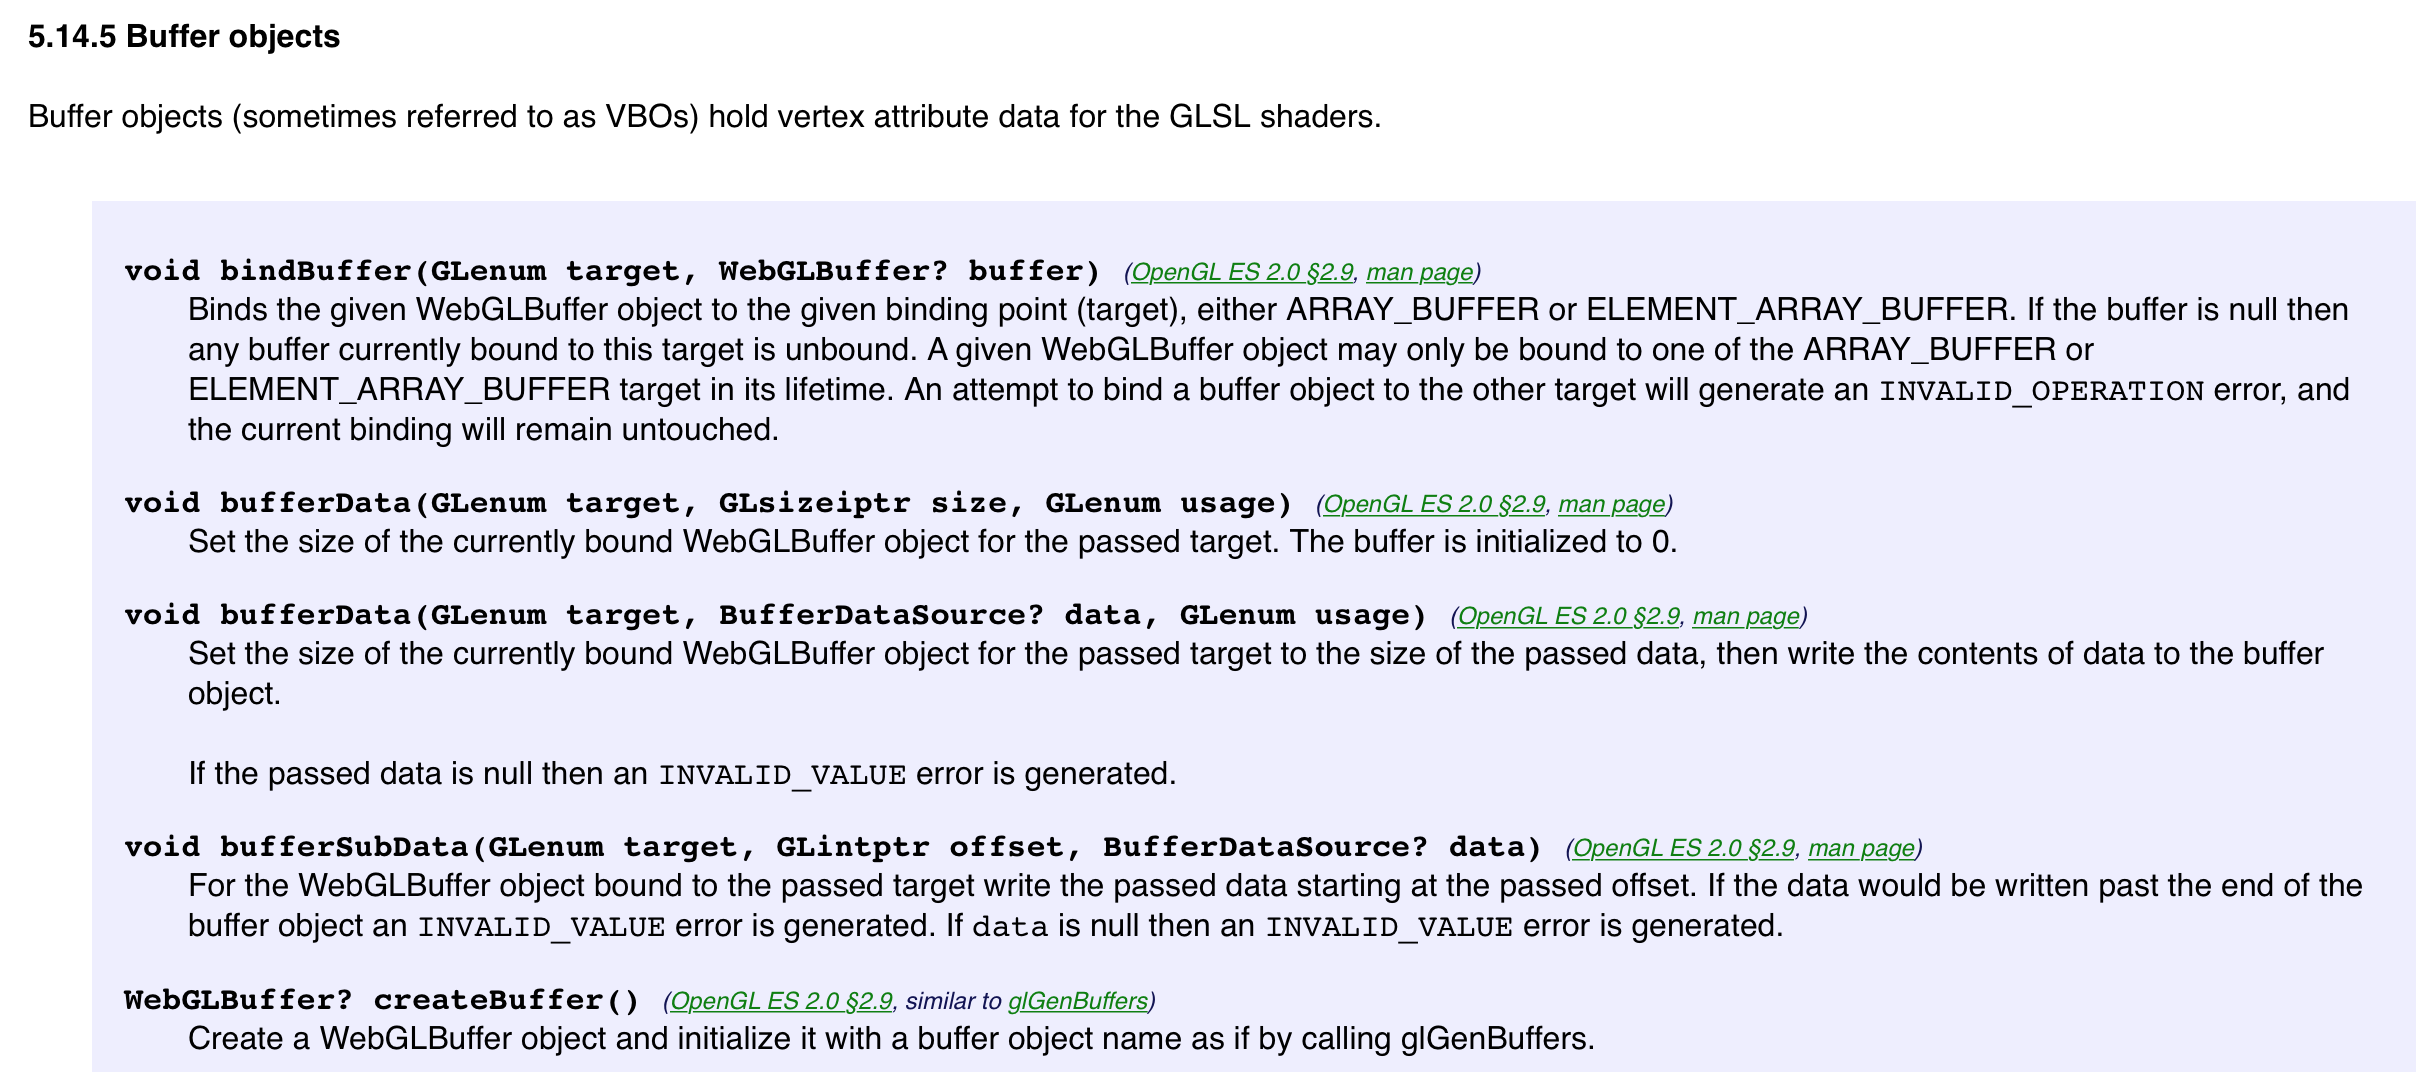
\includegraphics{images/webgl-spec.png}
\end{figure}

\paragraph{OpenGL ES}\label{opengl-es}

The
\href{https://www.khronos.org/registry/gles/specs/2.0/es_full_spec_2.0.25.pdf}{OpenGL
ES 2.0 spec} is a rather detailed specification. Some implementation
contrives are explained. So it is necessary for understanding the
browser implementation.

Here is a sample spec:

\begin{figure}[htbp]
\centering
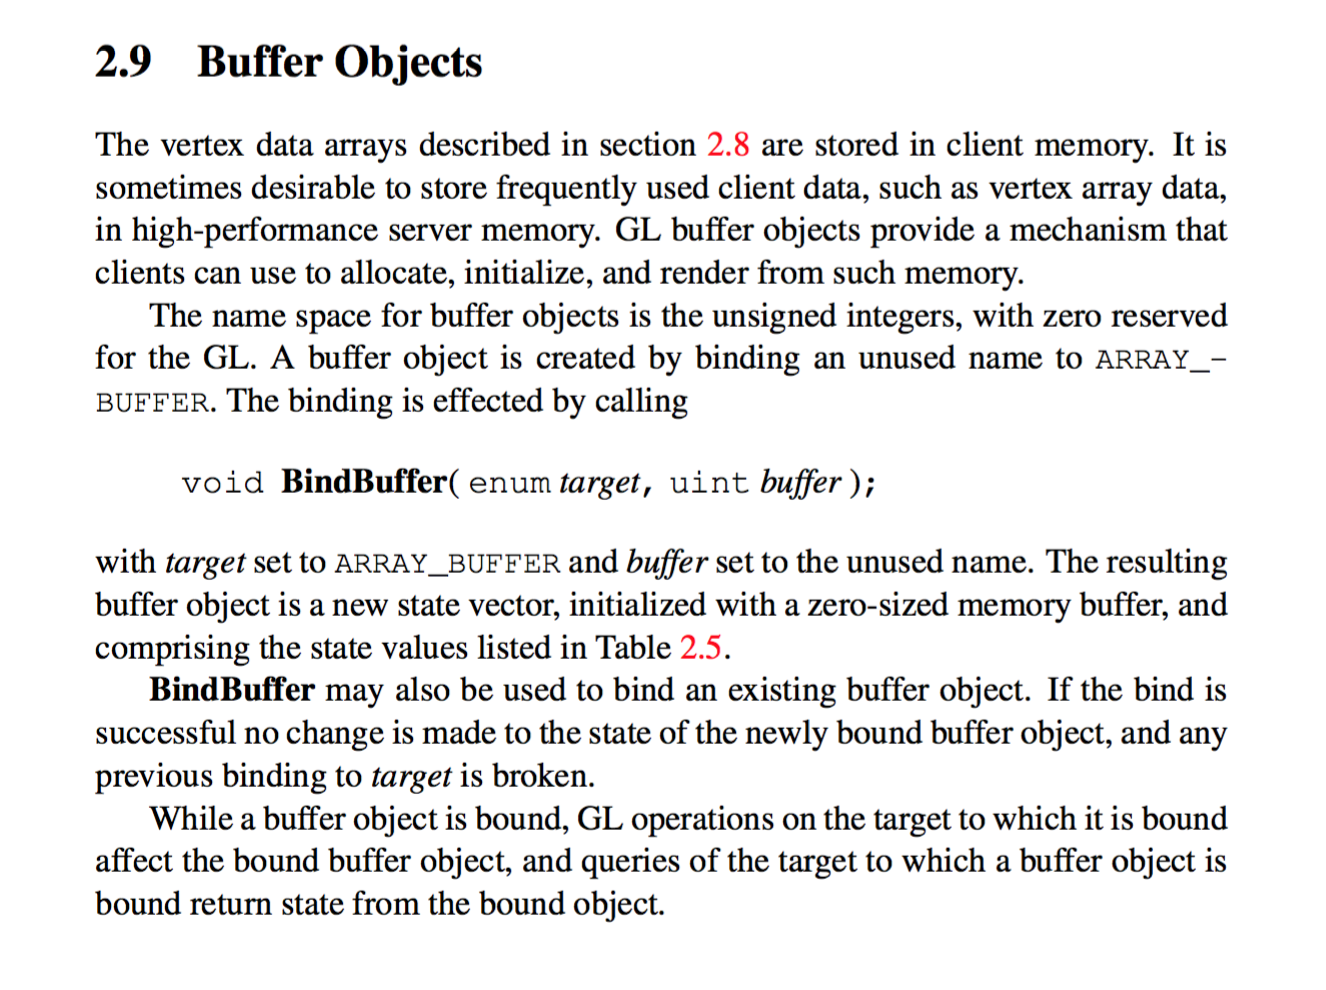
\includegraphics{images/opengl-spec.png}
\end{figure}

\paragraph{Example Implementation}\label{example-implementation}

As an example of implementation, we will see part of code in Firefox's
Browser Engine -- Gecko.

\begin{itemize}
\itemsep1pt\parskip0pt\parsep0pt
\item
  \href{https://github.com/mozilla/gecko-dev/blob/5a7da7930ebba958d98e2e42ed07d05c34d1873a/dom/webidl/WebGLRenderingContext.webidl}{\texttt{WebGLRenderingContext.webidl}}
\item
  \href{https://github.com/mozilla/gecko-dev/blob/71900c9741a8fafb137d9a57519dfa0fe280c4dc/gfx/angle/src/libANGLE/renderer/gl/RendererGL.h}{\texttt{RendererGL.h}}
\item
  \href{https://github.com/mozilla/gecko-dev/blob/7a82450687cc47dad34e3c89ca94cbd60bfd1aa6/dom/canvas/WebGLContextBuffers.cpp}{\texttt{WebGLContextBuffers.cpp}}
\end{itemize}

\subsubsection{Conformity status of popular
implementations}\label{conformity-status-of-popular-implementations}

Older but more completed from \cite{webglwiki}.

\paragraph{Desktop browsers}\label{desktop-browsers}

\begin{itemize}
\itemsep1pt\parskip0pt\parsep0pt
\item
  Google Chrome -- WebGL has been enabled on all platforms that have a
  capable graphics card with updated drivers since version 9, released
  in February 2011.
\item
  Mozilla Firefox -- WebGL has been enabled on all platforms that have a
  capable graphics card with updated drivers since version 4.0.
\item
  Safari -- Safari 6.0 and newer versions installed on OS X Mountain
  Lion, Mac OS X Lion and Safari 5.1 on Mac OS X Snow Leopard
  implemented support for WebGL, which was disabled by default before
  Safari 8.0.
\item
  Opera -- WebGL has been implemented in Opera 11 and 12, although was
  disabled by default in 2014.
\item
  Internet Explorer -- WebGL is partially supported in Internet Explorer
  11.
\item
  Microsoft Edge -- The initial stable release supports WebGL version
  0.95 (context name: ``experimental-webgl'').
\end{itemize}

\paragraph{Mobile browsers}\label{mobile-browsers}

\begin{itemize}
\itemsep1pt\parskip0pt\parsep0pt
\item
  BlackBerry 10 -- WebGL is available for BlackBerry devices since OS
  version 10.00
\item
  BlackBerry PlayBook -- WebGL is available via WebWorks and browser in
  PlayBook OS 2.00
\item
  Android Browser -- Basically unsupported.
\item
  Internet Explorer - WebGL is available on Windows Phone 8.1
\item
  Firefox for mobile -- WebGL is available for Android and MeeGo devices
  since Firefox 4.
\item
  Firefox OS
\item
  Google Chrome -- WebGL is available for Android devices since Google
  Chrome 25 and enabled by default since version 30.
\item
  Maemo -- In Nokia N900, WebGL is available in the stock microB browser
  from the PR1.2 firmware update onwards.
\item
  MeeGo - WebGL is unsupported in the stock browser ``Web.'' However, it
  is available through Firefox.
\item
  Opera Mobile - Opera Mobile 12 supports WebGL (on Android only).
\item
  Sailfish OS - WebGL is supported in the default Sailfish browser.
\item
  Tizen - WebGL is supported
\item
  Ubuntu Touch
\item
  WebOS
\item
  iOS -- WebGL is available for mobile Safari, in iOS 8.
\end{itemize}

\paragraph{More updated information}\label{more-updated-information}

You can check out the updated information in MDN \cite{webglmdn}

\begin{quote}
Support for WebGL is present in Firefox 4+, Google Chrome 9+, Opera 12+,
Safari 5.1+ and Internet Explorer 11+; however, the user's device must
also have hardware that supports these features.
\end{quote}

\subsection{Online API documentation}\label{online-api-documentation}

\begin{quote}
The junior developer read books and tutorials; The senior developers
read the API documentation; Only the platform developers and library
writers read the standards and specs.
\end{quote}

Why I should investigate into this part? The reason is simple: we want
to know \emph{how developer learns about the APIs and its intended
usage}.

Thus, we should pay attention to the following several things:

\begin{enumerate}
\def\labelenumi{\arabic{enumi}.}
\itemsep1pt\parskip0pt\parsep0pt
\item
  How does the single interface documentation look like?
\item
  Can developer find the usage of some particular functionality quick?
\item
  Is there enough but concise examples along side?
\item
  How is the edge cases and correctness issues mentioned?
\item
  How is the compatibility, security and performance issues mentioned?
\end{enumerate}

\subsubsection{Sources}\label{sources}

I found the MDN and MSDN have detailed API docs:

\begin{itemize}
\itemsep1pt\parskip0pt\parsep0pt
\item
  \href{https://developer.mozilla.org/en-US/docs/Web/API/WebGL_API}{Mozilla
  Developer Network}
\item
  \href{https://msdn.microsoft.com/en-us/library/dn621085(v=vs.85).aspx}{Microsoft
  Developer Network}
\end{itemize}

On the contrary, I don't find API doc about WebGL on
\href{https://www.chromium.org/developers}{Chromium's online
documentation};

\href{http://dev.opera.com}{Dev.Opera} has a lot of tutorials but not
API docs.

I find nothing significant on \href{https://developer.apple.com}{Apple
Developer site} either.

\subsubsection{Interface structure}\label{interface-structure}

\paragraph{MDN}\label{mdn}

For example,
\href{https://developer.mozilla.org/en-US/docs/Web/API/WebGLRenderingContext/copyTexImage2D}{copyTexImage2D}

There are short induction, syntax, parameters and return value
(semantics, types, ranges), examples, specification, browser
compatibility, related interfaces.

\paragraph{MSDN}\label{msdn}

Same example,
\href{https://msdn.microsoft.com/en-us/library/dn302380(v=vs.85).aspx}{copyTexImage2D}

Short intro, syntax, parameters and return value (semantics, more
explicit types, ranges), remarks, WebGL errors, related interfaces

\subsubsection{Usability}\label{usability}

The navigation of MDN is better than MSDN. And most of time the Google
will return MDN on searching a particular interface.

Also, the MDN provides per-interface examples and a lot of tutorials;
MSDN is short at this.

\subsubsection{Edge cases and
correctness}\label{edge-cases-and-correctness}

Both consider edge cases and special values. The MSDN has a WebGL errors
documentation, so it is more explicit about correctness.

\subsubsection{Compatibility, security and
performance}\label{compatibility-security-and-performance}

\paragraph{MDN}\label{mdn-1}

\begin{itemize}
\itemsep1pt\parskip0pt\parsep0pt
\item
  Compatibility: Information about conformity in all major desktop and
  mobile browsers.
\item
  Security: Not explicit
\item
  Performance: Not explicit
\end{itemize}

\paragraph{MSDN}\label{msdn-1}

\begin{itemize}
\itemsep1pt\parskip0pt\parsep0pt
\item
  Compatibility: Only one icon showing IE version supporting the
  interface.
\item
  Security: Not explicit
\item
  Performance: Not explicit
\end{itemize}

\subsection{Ecosystem}\label{ecosystem}

\subsubsection{Books}\label{books}

There are about 200 results returned for searching ``WebGL'' on
amazon.com. As a comparison, searching ``JavaScript'' gives you 9000+
results.

The most popular books are:

\subparagraph{\emph{WebGL Programming Guide: Interactive 3D Graphics
Programming with WebGL (OpenGL)} by Kouichi Matsuda and Rodger Lea
\cite{webglbook2013matsuda}:}\label{webgl-programming-guide-interactive-3d-graphics-programming-with-webgl-opengl-by-kouichi-matsuda-and-rodger-lea-webglbook2013matsuda}

\begin{quote}
You'll move from basic techniques such as rendering, animating, and
texturing triangles, all the way to advanced techniques such as fogging,
shadowing, shader switching, and displaying 3D models generated by
Blender or other authoring tools. This book won't just teach you WebGL
best practices, it will give you a library of code to jumpstart your own
projects.
\end{quote}

\subparagraph{\emph{Learning Three.js: The JavaScript 3D Library for
WebGL} by Jos Dirksen \cite{threejsbook2013dirksen}:}\label{learning-three.js-the-javascript-3d-library-for-webgl-by-jos-dirksen-threejsbook2013dirksen}

\begin{quote}
If you know JavaScript and want to start creating 3D graphics that run
in any browser, this book is a great choice for you. You don't need to
know anything about math or WebGL; all that you need is general
knowledge of JavaScript and HTML.
\end{quote}

\subparagraph{\emph{Programming 3D Applications with HTML5 and WebGL: 3D
Animation and Visualization for Web Pages} by Tony Parisi \cite{webglbook2014parisi}:}\label{programming-3d-applications-with-html5-and-webgl-3d-animation-and-visualization-for-web-pages-by-tony-parisi-webglbook2014parisi}

\begin{quote}
In two parts---Foundations and Application Development
Techniques---author Tony Parisi provides a thorough grounding in theory
and practice for designing everything from a simple 3D product viewer to
immersive games and interactive training systems. Ideal for developers
with Javascript and HTML experience.
\end{quote}

\subparagraph{\emph{WebGL: Up and Running} by Tony Parisi
\cite{webglbook2012parisi}:}\label{webgl-up-and-running-by-tony-parisi-webglbook2012parisi}

\begin{quote}
You don't have to be a game development wizard or have 3D graphics
experience to get started. If you use HTML, CSS, and JavaScript---and
have familiarity with JQuery and Ajax---this book will help you gain a
working knowledge of WebGL through clear and simple examples.
\end{quote}

\subparagraph{\emph{WebGL Insights} by Patrick Cozzi \cite{Cozzi15}:}\label{webgl-insights-by-patrick-cozzi-cozzi15}

\begin{quote}
WebGL Insights shares experience-backed lessons learned by the WebGL
community. It presents proven techniques that will be helpful to both
intermediate and advanced WebGL developers.
\end{quote}

It seems apparent that advanced materials share a high proportion. Also,
one books is not really teaching WebGL but Three.js.

These popular books' publication dated range from 2012 to 2015; In all
books, the newest is published in Feb 12, 2016 while the oldest is in
Oct 5, 2011 as I found.

\subsubsection{Tutorials}\label{tutorials}

Google gives me about 373,000 results for ``WebGL tutorial'' (28,900,000
for ``JavaScript'' at the same time).

The popular ones are:

\begin{enumerate}
\def\labelenumi{\arabic{enumi}.}
\itemsep1pt\parskip0pt\parsep0pt
\item
  \href{https://developer.mozilla.org/en-US/docs/Web/API/WebGL_API/Tutorial}{MDN
  tutorial}
\item
  \href{http://learningwebgl.com/blog/}{LearningWebGL}
\item
  \href{http://www.webglacademy.com}{WebGL Academy}
\item
  \href{https://webglfundamentals.org}{WebGL Fundamentals}
\end{enumerate}

\subsubsection{Misc}\label{misc}

\begin{itemize}
\itemsep1pt\parskip0pt\parsep0pt
\item
  High-level libraries: BabylonJS, three.js, O3D, OSG.JS, CopperLicht
  and GLGE
\item
  Game engines: Unreal Engine 4 and Unity 5
\item
  Languages:

  \begin{itemize}
  \itemsep1pt\parskip0pt\parsep0pt
  \item
    JavaScript (native)
  \item
    \href{http://typescript.away3d.com}{TypeScript}
  \item
    \href{https://github.com/jutaro/purescript-webgl}{PureScript}
  \item
    \href{http://www.coffeegl.com}{CoffeeScript}
  \item
    \href{http://haxor.xyz}{Haxe}
  \end{itemize}
\end{itemize}

\begin{figure}[h]
  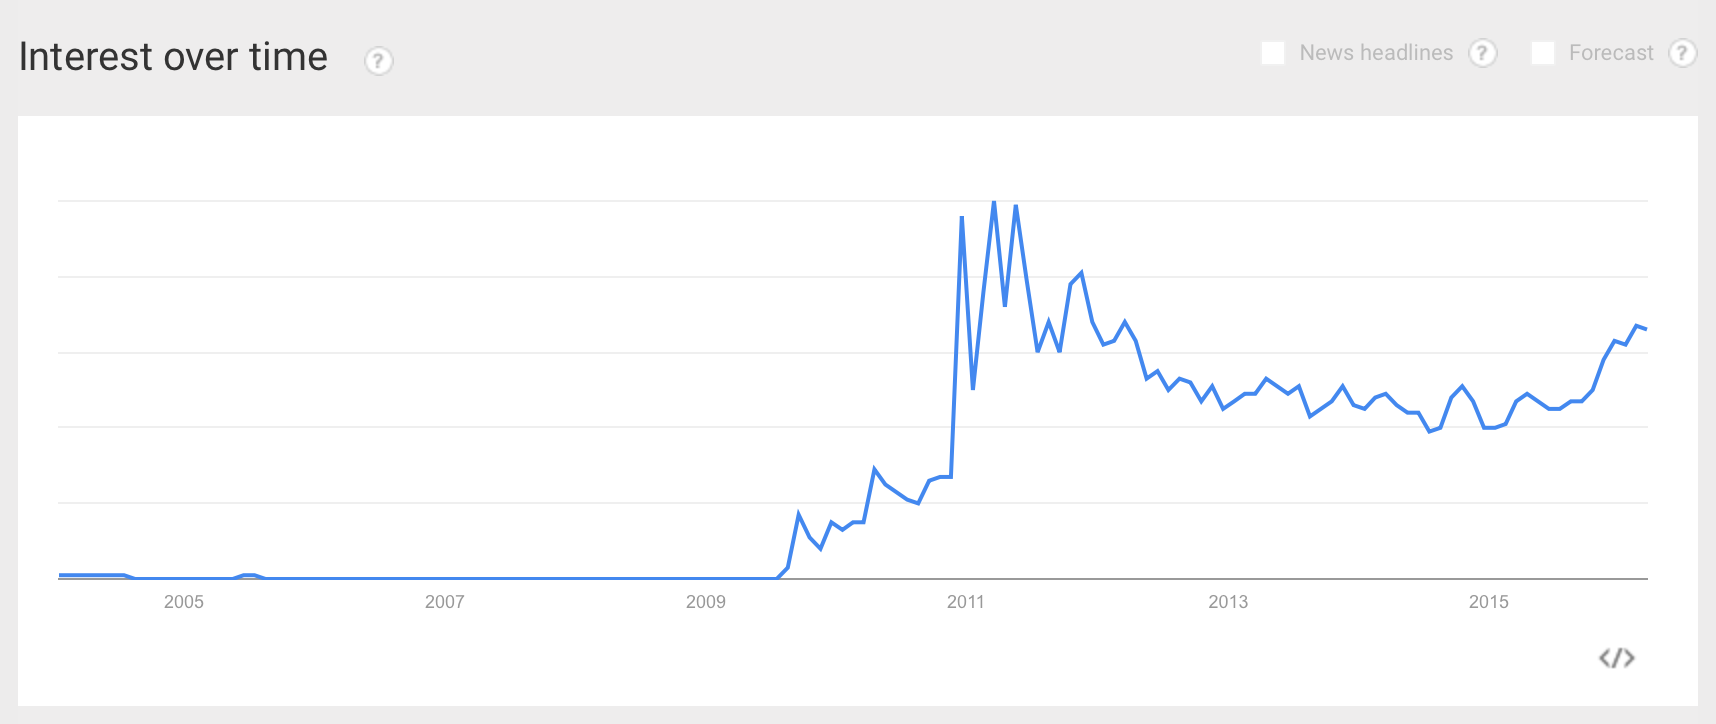
\includegraphics{images/trend.png}
  \caption{Google Trend for ``WebGL''}
\end{figure}

\subsection{Applications}\label{applications}

\subsubsection{Examples}\label{examples}

\begin{itemize}
\itemsep1pt\parskip0pt\parsep0pt
\item
  \href{http://eyes.nasa.gov/curiosity/}{NASA: Exploring Curiosity}
\item
  \href{https://www.chromeexperiments.com}{Chrome Experiments}
\item
  \href{http://threejs.org}{Three.js featured projects}
\end{itemize}

\subsubsection{Chrome Experiments}\label{chrome-experiments}

Currently, it has 567 experiments using WebGL. (About half of all
experiments).

From the first page, we will list the used technologies for each
application (only ones include WebGL), ``Open'' means it is
open-sourced.

\begin{enumerate}
\def\labelenumi{\arabic{enumi}.}
\itemsep1pt\parskip0pt\parsep0pt
\item
  \href{https://www.chromeexperiments.com/experiment/lines}{WebGL,
  Three.js, WebAudio; Open}
\item
  \href{https://www.chromeexperiments.com/experiment/gaze}{Javascript,WebGL,Three.js,GLSL,WebRTC,WebAudio}
\item
  \href{https://www.chromeexperiments.com/experiment/world}{Three.js,
  WebGL, Javascript}
\item
  \href{https://www.chromeexperiments.com/experiment/infinite-city}{Three.js,
  Javascript; Open}
\item
  \href{https://www.chromeexperiments.com/experiment/amalgame}{Javascript
  es6, WebGL, Three.js, Glsl}
\item
  \href{https://www.chromeexperiments.com/experiment/music-lab}{Web
  Audio API, Tone.JS, pixi.JS, WebGL, WebRTC; Open}
\item
  \href{https://www.chromeexperiments.com/experiment/medusae}{WebGL,
  WebAudio, Particulate.js, Three.js; Open}
\item
  \href{https://www.chromeexperiments.com/experiment/4dvj}{WebGL,
  Three.js, JavaScript (ES2015); Open}
\item
  \href{https://www.chromeexperiments.com/experiment/one-million-stars}{Javascript,
  WebGL, THREE.js, web audio API}
\end{enumerate}

So as we can see, Three.js is really popular; And half of them are open
sourced.

\subsubsection{Error and warnings
sampling}\label{error-and-warnings-sampling}

I tested the nine applications listed above, to see if there are any
errors or warnings in my browser (The experiment UA: Safari 9). Here is
the result for erros/warnings, and the rest is fine:

\begin{itemize}
\itemsep1pt\parskip0pt\parsep0pt
\item
  From 2nd app:
  \texttt{{[}Error{]} TypeError: undefined is not an object (evaluating 'camera.updateProjectionMatrix')}
\item
  From 3rd app:
  \texttt{{[}Warning{]} THREE.Material: 'envMap' parameter is undefined. (three.min.js, line 428)}
\item
  From 4th app:
  \texttt{{[}Warning{]} THREE.WebGLProgram: gl.getProgramInfoLog() – "WARNING: Output of vertex shader 'vNormal' not read by fragment shader↵" (three.js, line 29952)}
\item
  From 6th app:
  \texttt{{[}Warning{]} THREE.WebGLProgram: gl.getProgramInfoLog() – "WARNING: Output of vertex shader 'vPosition' not read by fragment shader↵"}
\end{itemize}

\newpage
\section{Troubles and
Trouble-Shooting}\label{troubles-and-trouble-shooting}

\subsection{Overview}\label{overview}

\subsubsection{Categories}\label{categories}

In typical WebGL applications, we might have following kinds of errors
(only the ones which \emph{will} happen every time, we don't count the
resource loading failure etc. in).

\begin{itemize}
\itemsep1pt\parskip0pt\parsep0pt
\item
  GLSL
\item
  Typo
\item
  unexpected parameter
\item
  Buffer not bound
\item
  GLSL
\item
  Resource deallocation
\item
  Lack of certain step
\item
  Buffer deallocation
\item
  Type error
\item
  Memory leak
\item
  Improper sharing
\item
  missing properties
\item
  Name not in scope
\item
  Undeclared identifier
\item
  Context management
\item
  Resource loading order
\item
  API usage error
\item
  Shader error
\item
  Threejs
\item
  Type errors
\item
  Matrix related
\item
  Others
\end{itemize}

\subsubsection{GLSL errors}\label{glsl-errors}

Referencing the GLSL errors in IE \cite{glerrormsdn}, we can divide GLSL
errors further into:

\begin{itemize}
\itemsep1pt\parskip0pt\parsep0pt
\item
  Internal compiler error
\item
  Compiler memory error - shader exceeds x bytes
\item
  Syntax error - x
\item
  Undeclared identifier x
\item
  Invalid arguments passed to function x
\item
  Postfix expression cannot be indexed
\item
  Index out of range
\item
  Incompatible index expression. For non-uniforms, the index must be an
  expression formed of the loop\_index and integer constants. For
  uniforms, the index must be an integer constant.
\item
  Index must be a constant
\item
  Argument x is not a sampler
\item
  Invalid macro name - cannot start with \texttt{GL\_} or contain
  \texttt{\_\_}
\item
  Incompatible types in expression
\item
  Expression in if statement does not evaluate to a boolean
\item
  Divide or mod by zero in constant expression
\item
  Invalid parameter count for macro
\item
  Maximum uniform vector count exceeded
\item
  Maximum attribute vector count exceeded
\item
  Maximum varying vector count exceeded
\item
  Maximum shader complexity exceeded
\item
  Identifier already declared
\item
  Invalid character used outside of comment
\item
  Invalid initializer in for loop, needs to be a single variable of type
  float or int and initialized to a constant
\item
  Invalid condition in for loop, needs to be in form
  \texttt{loop\_index \{ \&gt; \textbar{} \&gt;= \textbar{} \&lt; \textbar{} \&lt;= \textbar{} == \textbar{} != \} constant}
\item
  Invalid iteration in for loop, needs to be in form
  \texttt{\{ -\/-loop\_index \textbar{} ++loop\_index \textbar{} loop\_index++ \textbar{} loop\_index-\/- \textbar{} loop\_index+=constant \textbar{} loop\_index-=constant \}}
\item
  Invalid modification to loop index inside loop body
\item
  Invalid identifier name - cannot start with \texttt{gl\_},
  \texttt{webgl\_}, \texttt{\_webgl\_} or contain \texttt{\_\_}
\item
  Token exceeds maximum length
\item
  Invalid qualifier on array - cannot make arrays of attribute or const
  variables
\item
  Incompatible type used for return expression
\item
  Invalid qualifier on sampler variable declaration - must be uniform
\item
  Invalid type passed to matrix constructor - arguments must be a
  matrix, or a scalar / vector of float / int / bool
\item
  Invalid type passed to componentwise vector or matrix constructor -
  arguments must be a scalar / vector of float / int / bool
\item
  Invalid argument count in componentwise vector or matrix constructor -
  total components passed must equal vector or matrix size
\item
  Invalid expression on left of assignment expression
\item
  Invalid swizzle in field selection - swizzle component count must be
  equal or less than max vector size (4)
\item
  Invalid swizzle in field selection - swizzle components must be all
  from same set (xyzw, rgba or stpq)
\item
  Invalid swizzle component in field selection - must be from a valid
  GLSL set (xyzw, rgba or stpq)
\item
  Swizzle component out of range - must select a component that exists
  in the vector
\item
  This hardware is unable to support \texttt{gl\_FrontFacing}
\item
  Const variable requires initialization
\item
  Variables declared with uniform, attribute, or varying qualifier
  cannot be initialized
\item
  Varying variable cannot have bool, int, or struct type
\item
  Invalid argument passed to constructor - argument must be a basic GLSL
  type
\item
  Invalid type qualifier for function parameter - only const on in
  parameters is allowed
\item
  Array declarator requires a constant expression
\item
  Array was declared with size less than or equal to zero
\item
  Type qualifiers \texttt{uniform} and \texttt{attribute} are invalid
  for structs
\item
  Invalid field name for struct type
\item
  Invalid type for left hand side of field selection
\item
  Samplers are not allowed in structs
\item
  Macros must be redefined the same as original definition
\item
  Invalid loop index expression passed as out / inout parameter
\item
  Type cannot be used as a constructor
\item
  Undeclared type x
\item
  Embedded struct declarations are not allowed
\item
  Function x is declared and used but not defined
\item
  Function redefinition not allowed
\item
  Function redeclaration not allowed
\item
  Invalid single argument to vector constructor - must be a scalar type,
  or another vector, or a 2x2 matrix
\item
  Struct constructor arguments' types do not match the struct's field
  types
\item
  Invalid location for continue statment - must be inside of a loop
\item
  Cannot call main
\item
  Invalid qualifier on non-global variable - non-global variables can be
  const but cannot be varying, attribute or invariant
\item
  Cannot redefine main or define main with incorrect signature
\item
  Cannot use reserved operators such as \texttt{\textasciitilde{}},
  \texttt{\%=}, \texttt{\&gt;\&gt;=}, \texttt{\&lt;\&lt;=},
  \texttt{\&amp;=}, \texttt{\textbar{}=}, or \texttt{\^{}=}
\item
  Ternary conditional operator must have boolean expression for test
  condition
\item
  Ternary conditional operator must have two expressions of equal types
  after test condition
\item
  Invalid location for break statement - break statements must be inside
  a loop
\item
  Invalid location for discard statement - discard statements must be
  inside a fragment shader
\item
  Initializer for const variable must initialize to a constant value
\item
  Functions cannot be overloaded on return type
\item
  Known functions cannot be re-declared or re-defined
\item
  Function header definition parameter qualifiers must match declaration
  parameter qualifiers
\item
  Array size must be an integer constant expression
\item
  Array size expression too complex
\item
  \texttt{\#version} directive must specify 100 for version
\item
  \texttt{\#version} directive can only be preceded by whitespace or
  comments
\item
  Unary operator not defined for type
\item
  Struct declarations are disallowed in function parameter declarators
\item
  Struct type declaration exceeds maximum nesting level of
\item
  Operator not defined for struct types
\item
  Operator not defined for user-defined types that contain array types
\item
  Unknown extension: x
\item
  Invalid behavior specified for extension - behavior must be require,
  warn, enable or disable for regular extensions, or warn or disable for
  \texttt{all}
\item
  Required extension x is not supported
\item
  Preprocessor directives can only be preceded by whitespace on a line
\item
  Function declarations cannot be local
\item
  Variable declared as type void is not allowed
\item
  `void' is an invalid parameter type unless used as \texttt{(void)}
\end{itemize}

\subsection{Compiled Information from
MDN}\label{compiled-information-from-mdn}

Source: \href{https://developer.mozilla.org/en-US/docs/Web/API}{API},
\href{https://developer.mozilla.org/en-US/docs/Web/API/WebGL_API/WebGL_best_practices}{Best
Practices}

\subsubsection{Source of bugs}\label{source-of-bugs}

\paragraph{canvas element}\label{canvas-element}

To get the rendering context, i.e., the canvas element, we usually use
\texttt{getElementById} or similar way to fetch the DOM object. The
caveat is, the \texttt{id} is specified in HTML tag, such as

\begin{Shaded}
\begin{Highlighting}[]
\KeywordTok{<canvas}\OtherTok{ id=}\StringTok{"glcanvas"}\OtherTok{ width=}\StringTok{"640"}\OtherTok{ height=}\StringTok{"480"}\KeywordTok{>}
\end{Highlighting}
\end{Shaded}

And you must use the exact name in your JavaScript code. \textbf{It is
possible that you will type it wrongly or refer to another unrelated
canvas}.

\paragraph{\texttt{gl} Object}\label{gl-object}

\begin{Shaded}
\begin{Highlighting}[]
\KeywordTok{function} \FunctionTok{initWebGL}\NormalTok{(canvas) \{}
  \NormalTok{gl = }\KeywordTok{null}\NormalTok{;}

  \KeywordTok{try} \NormalTok{\{}
    \CommentTok{// Try to grab the standard context. If it fails, fallback to experimental.}
    \NormalTok{gl = }\OtherTok{canvas}\NormalTok{.}\FunctionTok{getContext}\NormalTok{(}\StringTok{"webgl"}\NormalTok{) || }\OtherTok{canvas}\NormalTok{.}\FunctionTok{getContext}\NormalTok{(}\StringTok{"experimental-webgl"}\NormalTok{);}
  \NormalTok{\}}
  \KeywordTok{catch}\NormalTok{(e) \{\}}

  \CommentTok{// If we don't have a GL context, give up now}
  \KeywordTok{if} \NormalTok{(!gl) \{}
    \FunctionTok{alert}\NormalTok{(}\StringTok{"Unable to initialize WebGL. Your browser may not support it."}\NormalTok{);}
    \NormalTok{gl = }\KeywordTok{null}\NormalTok{;}
  \NormalTok{\}}

  \KeywordTok{return} \NormalTok{gl;}
\NormalTok{\}}
\end{Highlighting}
\end{Shaded}

First, we might not have a functional \texttt{gl} (not \texttt{null})
always, which depends on the browser support. And second, in the
\texttt{getContext}, we are also forced to consider two standards.

\paragraph{Shader's source}\label{shaders-source}

The shader code is essentially a string. So as a result, you might
either define it in JavaScript, or store it as a HTML element, or even
request it as a resource dynamically from other address.

\begin{Shaded}
\begin{Highlighting}[]
\KeywordTok{if} \NormalTok{(!}\OtherTok{gl}\NormalTok{.}\FunctionTok{getProgramParameter}\NormalTok{(shaderProgram, }\OtherTok{gl}\NormalTok{.}\FunctionTok{LINK_STATUS}\NormalTok{)) \{}
  \FunctionTok{alert}\NormalTok{(}\StringTok{"Unable to initialize the shader program."}\NormalTok{);}
\NormalTok{\}}
\end{Highlighting}
\end{Shaded}

The above snippet checks if the \texttt{gl.linkProgram} calling succeeds
by checking if return value is \texttt{null}. It is apparently something
easy to forget.

\paragraph{Attribute names}\label{attribute-names}

The shader code will use some variable to communicate with JavaScript.
For example

\begin{verbatim}
<script id="shader-vs" type="x-shader/x-vertex">
  attribute vec3 aVertexPosition;

  uniform mat4 uMVMatrix;
  uniform mat4 uPMatrix;

  void main(void) {
    gl_Position = uPMatrix * uMVMatrix * vec4(aVertexPosition, 1.0);
  }
</script>
\end{verbatim}

On the JavaScript side, we have to

\begin{Shaded}
\begin{Highlighting}[]
\CommentTok{// During Shader initialization}
\NormalTok{vertexPositionAttribute = }\OtherTok{gl}\NormalTok{.}\FunctionTok{getAttribLocation}\NormalTok{(shaderProgram, }\StringTok{"aVertexPosition"}\NormalTok{);}
\OtherTok{gl}\NormalTok{.}\FunctionTok{enableVertexAttribArray}\NormalTok{(vertexPositionAttribute);}

\CommentTok{// During scene rendering}
\KeywordTok{var} \NormalTok{pUniform = }\OtherTok{gl}\NormalTok{.}\FunctionTok{getUniformLocation}\NormalTok{(shaderProgram, }\StringTok{"uPMatrix"}\NormalTok{);}
\OtherTok{gl}\NormalTok{.}\FunctionTok{uniformMatrix4fv}\NormalTok{(pUniform, }\KeywordTok{false}\NormalTok{, }\KeywordTok{new} \FunctionTok{Float32Array}\NormalTok{(}\OtherTok{perspectiveMatrix}\NormalTok{.}\FunctionTok{flatten}\NormalTok{()));}

\KeywordTok{var} \NormalTok{mvUniform = }\OtherTok{gl}\NormalTok{.}\FunctionTok{getUniformLocation}\NormalTok{(shaderProgram, }\StringTok{"uMVMatrix"}\NormalTok{);}
\OtherTok{gl}\NormalTok{.}\FunctionTok{uniformMatrix4fv}\NormalTok{(mvUniform, }\KeywordTok{false}\NormalTok{, }\KeywordTok{new} \FunctionTok{Float32Array}\NormalTok{(}\OtherTok{mvMatrix}\NormalTok{.}\FunctionTok{flatten}\NormalTok{()));}

\OtherTok{gl}\NormalTok{.}\FunctionTok{bindBuffer}\NormalTok{(}\OtherTok{gl}\NormalTok{.}\FunctionTok{ARRAY_BUFFER}\NormalTok{, squareVerticesBuffer);}
\OtherTok{gl}\NormalTok{.}\FunctionTok{vertexAttribPointer}\NormalTok{(vertexPositionAttribute, }\DecValTok{3}\NormalTok{, }\OtherTok{gl}\NormalTok{.}\FunctionTok{FLOAT}\NormalTok{, }\KeywordTok{false}\NormalTok{, }\DecValTok{0}\NormalTok{, }\DecValTok{0}\NormalTok{);}
\end{Highlighting}
\end{Shaded}

So, we have to match the names (i.e. \texttt{aVertexPosition},
\texttt{uPMatrix} and \texttt{uMVMatrix} in the above example) in two
language domains, both in syntax and semantics.

\paragraph{Array}\label{array}

This is how to fill data into GL buffer:
\texttt{gl.bufferData(gl.ELEMENT\_ARRAY\_BUFFER, new Uint16Array(cubeVertexIndices), gl.STATIC\_DRAW);}

The \texttt{Uint16Array} is a raw, platform-dependent way of storing an
array of data. Similarly, we also have \texttt{Array},
\texttt{Int8Array}, \texttt{Float32Array} \ldots{}

Interestingly, let compare it with OpenGL ES interface:
\texttt{void BufferData( enum target, sizeiptr size, const void *data, enum usage );}.

You can see that, the \texttt{Uint16} array could be translated into a
raw array and a element size indicator.

\subsubsection{Things to avoid}\label{things-to-avoid}

\begin{itemize}
\itemsep1pt\parskip0pt\parsep0pt
\item
  You should never use \texttt{\#ifdef GL\_ES} in your WebGL shaders;
  although some early examples used this, it's not necessary, since this
  condition is always true in WebGL shaders.
\item
  Using \texttt{high} precision in fragment shaders will prevent your
  content from working on some older mobile hardware. You can use
  \texttt{medium} instead, but be aware that this often results in
  corrupted rendering due to lack of precision on most mobile devices,
  and the corruption is not going to be visible on a typical desktop
  computer. In general, only using \texttt{high} in both vertex and
  fragment shaders is safer unless shaders are thoroughly tested on a
  variety of platforms. Starting in Firefox 11, the WebGL
  \texttt{getShaderPrecisionFormat()} function is implemented, allowing
  you to check if \texttt{high} precision is supported, and more
  generally letting you query the actual precision of all supported
  precision qualifiers.
\item
  Anything that requires syncing the CPU and GPU sides is potentially
  very slow, so if possible you should try to avoid doing that in your
  main rendering loops. This includes the following WebGL calls:
  \texttt{getError()}, \texttt{readPixels()}, and \texttt{finish()}.
  WebGL getter calls such as \texttt{getParameter()} and
  \texttt{getUniformLocation()} should be considered slow too, so try to
  cache their results in a JavaScript variable.
\item
  Simpler shaders perform better than complex ones. In particular, if
  you can remove an \texttt{if} statement from a shader, that will make
  it run faster. Division and math functions like \texttt{log()} should
  be considered expensive too.
\item
  Always have vertex attrib 0 array enabled. If you draw with vertex
  attrib 0 array disabled, you will force the browser to do complicated
  emulation when running on desktop OpenGL (e.g.~on Mac OS X). This is
  because in desktop OpenGL, nothing gets drawn if vertex attrib 0 is
  not array-enabled. You can use \texttt{bindAttribLocation()} to force
  a vertex attribute to use location 0, and use
  \texttt{enableVertexAttribArray()} to make it array-enabled.
\end{itemize}

\subsection{Compiled Information from
Stackoverflow}\label{compiled-information-from-stackoverflow}

\href{http://stackoverflow.com/search?q=WebGL}{Source}

\subsubsection{Examples}\label{examples-1}

\paragraph{Undeclared identifier}\label{undeclared-identifier}

\begin{itemize}
\itemsep1pt\parskip0pt\parsep0pt
\item
  \href{http://stackoverflow.com/questions/4468329/gl-color-is-undeclared-identifier-on-webgl}{gl-color-is-undeclared-identifier-on-webgl}
\end{itemize}

\paragraph{Context management}\label{context-management}

\begin{itemize}
\itemsep1pt\parskip0pt\parsep0pt
\item
  \href{http://stackoverflow.com/questions/27544729/three-js-error-creating-webgl-context}{another
  \texttt{canvas.getContext('2d')} occupied this canvas context.}
\item
  \href{http://stackoverflow.com/questions/25219352/webgl-scene-doest-render-because-of-lost-context}{webgl-scene-doest-render-because-of-lost-context}
\end{itemize}

\paragraph{Resource loading order}\label{resource-loading-order}

\begin{itemize}
\itemsep1pt\parskip0pt\parsep0pt
\item
  \href{http://stackoverflow.com/questions/14943148/webgl-getattriblocation-no-object-shader-issue}{Try
  to render the scene before the shader program is downloaded and
  compiled}
\end{itemize}

\paragraph{API usage error}\label{api-usage-error}

\begin{itemize}
\itemsep1pt\parskip0pt\parsep0pt
\item
  \href{http://stackoverflow.com/questions/33725228/webgl-fragment-shader-constructor-error-too-many-arguments}{WebGL
  Fragment Shader constructor error - Too many arguments}
\item
  \href{http://stackoverflow.com/questions/28490041/webgl-vbo-error-in-firefox}{Where
  is your setup code}
\item
  \href{http://stackoverflow.com/questions/32618792/webgl-error-when-attempting-to-get-color-data-from-vec4}{WebGL
  error when attempting to get color data from vec4}
\item
  \href{http://stackoverflow.com/questions/26544800/simple-triangle-in-webgl}{API
  name typo}
\item
  \href{http://stackoverflow.com/questions/21436678/what-is-wrong-with-this-webgl-code}{what-is-wrong-with-this-webgl-code}
\item
  \href{http://stackoverflow.com/questions/33057640/why-my-mutiple-animated-objects-are-not-displayed-by-my-code-webgl}{Because
  \texttt{createProgram} don't return anything}
\item
  \href{http://stackoverflow.com/questions/19758786/webgl-keep-previous-object}{should
  be calling \texttt{gl.drawArrays()} once for every object that is
  currently on the screen}
\item
  \href{http://stackoverflow.com/questions/17316171/webgl-drawarrays-attribs-not-setup-correctly}{have
  to create an array buffer for each object you are drawing}
\item
  \href{http://stackoverflow.com/questions/32447641/what-is-common-cause-of-range-out-of-bounds-of-buffer-in-webgl}{3
  reasons of failing to call \texttt{gl.drawElements}}
\item
  \href{http://stackoverflow.com/questions/8900559/webgl-drawarrays-with-invalid-mode-is-not-generating-a-error}{webgl-drawarrays-with-invalid-mode-is-not-generating-a-error}
\item
  \href{http://stackoverflow.com/questions/15751791/webgl-drawelements-out-of-range}{webgl-drawelements-out-of-range}
\item
  \href{http://stackoverflow.com/questions/31750163/webgl-failing-at-drawing-points-gldrawarrays-attempt-to-access-out-of-range}{webgl-failing-at-drawing-points-gldrawarrays-attempt-to-access-out-of-range}
\item
  \href{http://stackoverflow.com/questions/14641618/webgl-invalid-value-attachshader-no-object-or-object-deleted-is-this-secretl}{webgl-invalid-value-attachshader-no-object-or-object-deleted-is-this-secretl}
\item
  \href{http://stackoverflow.com/questions/34617490/why-doesnt-my-sphere-render-complete}{why-doesnt-my-sphere-render-complete}
\item
  \href{http://stackoverflow.com/questions/15751791/webgl-drawelements-out-of-range/15753839\#15753839}{webgl-drawelements-out-of-range}
\item
  \href{http://stackoverflow.com/questions/11998781/webgl-invalid-operation-useprogram/11998987\#11998987}{webgl-invalid-operation-useprogram}
\item
  \href{http://stackoverflow.com/questions/32115328/type-canvasrenderingcontext2d-webglrenderingcontext-is-not-assignable-to-typ/32116589\#32116589}{type-canvasrenderingcontext2d-webglrenderingcontext-is-not-assignable-to-typ}
\item
  \href{http://stackoverflow.com/questions/11216912/webgl-shader-errors/11217704\#11217704}{webgl-shader-errors}
\item
  \href{http://stackoverflow.com/questions/21128464/what-will-happen-if-an-attribute-is-used-in-program-without-enabled-and-binding}{what-will-happen-if-an-attribute-is-used-in-program-without-enabled-and-binding}
\item
  \href{http://stackoverflow.com/questions/21200386/webgl-gl-error-gl-invalid-operation-gldrawelements-attempt-to-access-out-of/21212640\#21212640}{webgl-gl-error-gl-invalid-operation-gldrawelements-attempt-to-access-out-of}
\end{itemize}

\paragraph{Shader error}\label{shader-error}

\begin{itemize}
\itemsep1pt\parskip0pt\parsep0pt
\item
  \href{http://stackoverflow.com/questions/20821486/how-to-debug-webgl-uncaught-type-error}{\texttt{uniform1i(3, 0)}
  Is not valid WebGL}
\item
  \href{http://stackoverflow.com/questions/31690465/webgl-shaders-uncaught-syntax-error}{GLSL
  interpreted as javascript}
\item
  \href{http://stackoverflow.com/questions/18500831/webgl-compileshader-syntax-error}{WebGL
  - compileShader syntax error}
\item
  \href{http://stackoverflow.com/questions/11216912/webgl-shader-errors}{WebGL
  shader errors}
\item
  \href{http://stackoverflow.com/questions/23724507/webgl-unable-to-initialize-shader-program}{webgl-unable-to-initialize-shader-program}
\item
  \href{http://stackoverflow.com/questions/20084865/google-chrome-webgl-shader-compile-linker-error-uniforms-with-the-same-name-but}{google-chrome-webgl-shader-compile-linker-error-uniforms-with-the-same-name-but}
\item
  \href{http://stackoverflow.com/questions/31520908/wrong-integer-math-in-webgl-shaders}{wrong-integer-math-in-webgl-shaders}
\item
  \href{http://stackoverflow.com/questions/12755044/shader-compile-errors}{shader-compile-errors}
\item
  \href{http://stackoverflow.com/questions/18815502/using-a-uniform-in-an-if-instruction-inside-a-fragment-shader-dont-work-since}{using-a-uniform-in-an-if-instruction-inside-a-fragment-shader-dont-work-since}
\item
  \href{http://stackoverflow.com/questions/23724507/webgl-unable-to-initialize-shader-program/23740067\#23740067}{webgl-unable-to-initialize-shader-program}
\item
  \href{http://stackoverflow.com/questions/31665132/gl-invalid-operation-caused-by-samplercube}{gl-invalid-operation-caused-by-samplercube}
\end{itemize}

\paragraph{Threejs}\label{threejs}

\begin{itemize}
\itemsep1pt\parskip0pt\parsep0pt
\item
  \href{http://stackoverflow.com/questions/24635753/three-js-webgl-error-drawing-texture-on-a-plane}{Three.js:
  WebGL (error) drawing texture on a plane}
\item
  \href{http://stackoverflow.com/questions/14842857/normalize-function-in-webgl-not-working-three-js}{Normalize
  takes a vec3 not a vec4}
\item
  \href{http://stackoverflow.com/questions/29059306/three-js-webgl-invalid-operation-bindtexture-object-not-from-this-context}{three-js-webgl-invalid-operation-bindtexture-object-not-from-this-context}
\item
  \href{http://stackoverflow.com/questions/30074972/canvas-renderer-not-working}{canvas-renderer-not-working}
\item
  \href{http://stackoverflow.com/questions/11359152/three-js-particlesystem-creation-gives-invalid-operation-not-bound-buffer-array}{three-js-particlesystem-creation-gives-invalid-operation-not-bound-buffer-array}
\end{itemize}

\paragraph{Others}\label{others}

\begin{itemize}
\itemsep1pt\parskip0pt\parsep0pt
\item
  \href{http://stackoverflow.com/questions/26400009/webgl-get-error-warning-message-text-as-a-string}{WebGL:
  get error/warning message text as a string}
\item
  \href{http://stackoverflow.com/questions/22666556/webgl-texture-creation-trouble}{WebGL
  texture creation trouble}
\item
  \href{http://stackoverflow.com/questions/28604747/understanding-webgl-state}{Understanding
  WebGL State}
\item
  \href{http://stackoverflow.com/questions/19829244/problems-with-texture-array-sending-to-shaders-in-webgl}{problems-with-texture-array-sending-to-shaders-in-webgl}
\item
  \href{http://stackoverflow.com/questions/31433319/webgl-rendering-an-float32array-of-a-lot-of-elements-showing-out-of-range-vertic}{webgl-rendering-an-float32array-of-a-lot-of-elements-showing-out-of-range-vertic}
\item
  \href{http://stackoverflow.com/questions/21537721/array-buffer-not-working-with-webgl}{array-buffer-not-working-with-webgl}
\item
  \href{http://stackoverflow.com/questions/27524490/webgl-texture-is-not-showing-correctly/27525037\#27525037}{webgl-texture-is-not-showing-correctly}
\item
  \href{http://stackoverflow.com/questions/26134077/passing-color-to-fragment-shader-from-javascript}{passing-color-to-fragment-shader-from-javascript}
\item
  \href{http://stackoverflow.com/questions/4009914/is-there-a-lint-tool-for-opengl-shading-language/4017112\#4017112}{is-there-a-lint-tool-for-opengl-shading-language}
\item
  \href{http://stackoverflow.com/questions/17035588/three-js-shader-extention-errors}{three-js-shader-extention-errors}
\end{itemize}

\paragraph{Type errors}\label{type-errors}

\begin{itemize}
\itemsep1pt\parskip0pt\parsep0pt
\item
  \href{http://stackoverflow.com/questions/28747458/webgl-invalid-operation-vertexattribpointer-stride-or-offset-not-valid-for-ty}{webgl-invalid-operation-vertexattribpointer-stride-or-offset-not-valid-for-ty}
\item
  \href{http://stackoverflow.com/questions/10590819/webgl-glsl-shader-accessing-texture2d-overrides-other-texture/10592100\#10592100}{webgl-glsl-shader-accessing-texture2d-overrides-other-texture}
\item
  \href{http://stackoverflow.com/questions/31429591/webgl-code-not-working}{So
  finally it is a typing mistake}
\end{itemize}

\paragraph{Matrix related}\label{matrix-related}

\begin{itemize}
\itemsep1pt\parskip0pt\parsep0pt
\item
  \href{http://stackoverflow.com/questions/14784427/webgl-using-gl-matrix-library-mat4-translate-not-running}{webgl-using-gl-matrix-library-mat4-translate-not-running}
\item
  \href{http://stackoverflow.com/questions/17345432/square-doesnt-appear-using-perspective-matrix}{square-doesnt-appear-using-perspective-matrix}
\end{itemize}

\subsection{Compiled Information from
three.js}\label{compiled-information-from-three.js}

\subsubsection{Overview}\label{overview-1}

\begin{itemize}
\itemsep1pt\parskip0pt\parsep0pt
\item
  threejs-issue-5421: Buffer deallocation
\item
  threejs-issue-5569: Type mismatch
\item
  threejs-issue-5680: Memory leak
\item
  threejs-issue-5871: Improper sharing
\item
  threejs-issues-83: Name not in scope
\item
  threejs-pull-1602: GLSL
\item
  threejs-issue-4834: Unexpected parameter
\item
  threejs-issue-5098: Buffer not bound
\item
  threejs-issue-5196: Buffer not bound
\item
  threejs-issue-5222: GLSL \& Unexpected parameter
\item
  threejs-issue-5269: Resource deallocation
\item
  threejs-issue-5293: Lack of certain step
\item
  threejs-issue-6952: Missing properties
\item
  threejs-issue-6956: GLSL
\end{itemize}

\subsubsection{Details}\label{details}
\subsubsection{threejs-pull-1602}\label{threejs-pull-1602}

\subparagraph{Categories}\label{categories}

\begin{itemize}
\itemsep1pt\parskip0pt\parsep0pt
\item
  GLSL
\end{itemize}

\subparagraph{Link}\label{link}

\url{https://github.com/mrdoob/three.js/pull/1602}

\subparagraph{Remark}\label{remark}

This PR mentioned a problem about adding precision qualifiers to resolve
shader compilation errors on mobile device. This is also a nasty problem
which is platform-dependent

\paragraph{threejs-issue-1329}\label{threejs-issue-1329}

\subparagraph{Categories}\label{categories-1}

\begin{itemize}
\itemsep1pt\parskip0pt\parsep0pt
\item
  Typo
\end{itemize}

\subparagraph{Link}\label{link-1}

\url{https://github.com/mrdoob/three.js/issues/1329}

\subparagraph{Remark}\label{remark-1}

\texttt{THREE.UnsignedIntType} is written wrongly as
\texttt{THREE.UnsignedShortType}. However, its namespace is
\texttt{THREE}, which is defined by library, not by WebGL.

\subparagraph{Possible fix}\label{possible-fix}

I think TAJS might be able to resolve this by analyzing information of
object property?

\paragraph{threejs-issue-4834}\label{threejs-issue-4834}

\subparagraph{Categories}\label{categories-2}

\begin{itemize}
\itemsep1pt\parskip0pt\parsep0pt
\item
  unexpected parameter
\end{itemize}

\subparagraph{Link}\label{link-2}

\url{https://github.com/mrdoob/three.js/issues/4834}

\subparagraph{Remark}\label{remark-2}

Discussed 2 problems here related to the compilation failure of the
shader.

\begin{verbatim}
            - [This commit](https://github.com/Nimanf/three.js/commit/7f7650c5e012890a34c26c1c6fa2f8482d855627) used `max()` to limit negative values for `pow()` in shaders.

            - Then there is a discussion about the warning X3557 caused by `MAX_DIR_LIGHTS` is 1 and the redundant loop:
              ```
              #define MAX_DIR_LIGHTS 1
              #if MAX_DIR_LIGHTS > 0
              for( int i = 0; i < MAX_DIR_LIGHTS; i++ ) { ...
              ```
\end{verbatim}

\subparagraph{Possible fix}\label{possible-fix-1}

maybe same as
\href{https://git.ustclug.org/VeriGL/VeriGL-Dark-Side/wikis/threejs-issue-5222}{threejs
issue 5222}

\paragraph{threejs-issue-5098}\label{threejs-issue-5098}

\subparagraph{Categories}\label{categories-3}

\begin{itemize}
\itemsep1pt\parskip0pt\parsep0pt
\item
  Buffer not bound
\end{itemize}

\subparagraph{Link}\label{link-3}

\url{https://github.com/mrdoob/three.js/issues/5098}

\subparagraph{Remark}\label{remark-3}

An eye catched error.

\begin{quote}
\texttt{THREE.Float32Attribute} has been removed.
\end{quote}

Use THREE.BufferAttribute( array, itemSize ) instead.

this
\href{https://github.com/mrdoob/three.js/commit/e5b1d38e1e90bc9f7b16da7c1e53e66c5e8c2178}{commit}
solves this:

\begin{verbatim}
- geometry.addAttribute( 'position', new THREE.Float32Attribute( numEdges * 2 * 3, 3 ) );
+  geometry.addAttribute( 'position', new THREE.BufferAttribute( new Float32Array( numEdges * 2 * 3 ), 3 ) );
\end{verbatim}

\subparagraph{Possible fix}\label{possible-fix-2}

Search for available functions in the lib

\paragraph{threejs-issue-5196}\label{threejs-issue-5196}

\subparagraph{Categories}\label{categories-4}

\begin{itemize}
\itemsep1pt\parskip0pt\parsep0pt
\item
  Buffer not bound
\end{itemize}

\subparagraph{Link}\label{link-4}

\url{https://github.com/mrdoob/three.js/issues/5196\#issue-40214568}

\subparagraph{Remark}\label{remark-4}

Found while playing with threejs.org/editor

After adding a Mesh with the Menubar's `Add' panel, sidebar geometry
parameter changes cause the object to stop displaying.

Console warnings from WebGL:
\texttt{WebGL: INVALID\_OPERATION: vertexAttribPointer: no bound ARRAY\_BUFFER three.min.js:545 WebGL: INVALID\_OPERATION: vertexAttribPointer: no bound ARRAY\_BUFFER three.min.js:549 WebGL: INVALID\_OPERATION: drawElements: no ELEMENT\_ARRAY\_BUFFER bound three.min.js:552 {[}17:54:37{]} Saved state to IndexedDB. 0.71ms Storage.js:64}

\subparagraph{Possible fix}\label{possible-fix-3}

Track the \texttt{gl} context and the \texttt{buffer} might avoid these.

\paragraph{threejs-issue-5222}\label{threejs-issue-5222}

\subparagraph{Categories}\label{categories-5}

\begin{itemize}
\itemsep1pt\parskip0pt\parsep0pt
\item
  GLSL
\item
  unexpected parameter
\end{itemize}

\subparagraph{Link}\label{link-5}

\url{https://github.com/mrdoob/three.js/issues/5222}

\subparagraph{Remark}\label{remark-5}

As referred to to
\href{https://www.khronos.org/registry/gles/specs/2.0/GLSL_ES_Specification_1.0.17.pdf}{GLSL
mannual} P65, in \texttt{genType pow (genType x, genType y)}, results
are undefined if x = 0 and y \textless{}= 0. So in the generated GLSL in
the issue, \texttt{pow(pointDotNormalHalf, shininess)} could be
undefined and not warned. In the commit
\href{https://github.com/mrdoob/three.js/commit/a13cf4343effc741b0aa333c37062cc7cc3d71c7}{\#7252},
this was fixed by:
\texttt{-    uniforms.shininess.value = material.shininess;}
\texttt{+    uniforms.shininess.value = Math.max( material.shininess, 1e-4 );}

\subparagraph{Possible fix}\label{possible-fix-4}

Interval analysis and warning

\subparagraph{Related}\label{related}

\begin{itemize}
\itemsep1pt\parskip0pt\parsep0pt
\item
  \href{https://github.com/mrdoob/three.js/issues/7252}{messed up OBJMTL
  loader \#7252}
\item
  \href{https://github.com/mrdoob/three.js/issues/6057}{MeshPhongMaterial
  with shininess = 0 causes artifacts on Windows \#6057}
\end{itemize}

\paragraph{threejs-issue-5269}\label{threejs-issue-5269}

\subparagraph{Categories}\label{categories-6}

\begin{itemize}
\itemsep1pt\parskip0pt\parsep0pt
\item
  Resource deallocation
\end{itemize}

\subparagraph{Link}\label{link-6}

\url{https://github.com/mrdoob/three.js/issues/5269}

\subparagraph{Remark}\label{remark-6}

The child of object3D was not removed before removing the object3D
itself. This arouse the memory leakage.

\subparagraph{Possible fix}\label{possible-fix-5}

Might be fixed by tracking the state of the object?

\paragraph{threejs-issue-5293}\label{threejs-issue-5293}

\subparagraph{Categories}\label{categories-7}

\begin{itemize}
\itemsep1pt\parskip0pt\parsep0pt
\item
  Lack of certain step
\end{itemize}

\subparagraph{Link}\label{link-7}

\url{https://github.com/mrdoob/three.js/issues/5293}

\subparagraph{Remark}\label{remark-7}

\texttt{WebGLRenderer} is not doing \texttt{updateObject( object )}
because is not visible from the main camera. hen an error
\texttt{glDrawElements: range out of bounds for buffer} would occur.

\subparagraph{Possible fix}\label{possible-fix-6}

Might be fixed by tracking the state of the object?

\subparagraph{Related}\label{related-1}

\begin{itemize}
\itemsep1pt\parskip0pt\parsep0pt
\item
  The author broke it again recently in
  \href{https://github.com/mrdoob/three.js/issues/6996}{\#6996}
\end{itemize}

\paragraph{threejs-issue-5421}\label{threejs-issue-5421}

\subparagraph{Categories}\label{categories-8}

\begin{itemize}
\itemsep1pt\parskip0pt\parsep0pt
\item
  Buffer deallocation
\end{itemize}

\subparagraph{Link}\label{link-8}

\url{https://github.com/mrdoob/three.js/issues/5421}

\subparagraph{Remark}\label{remark-8}

According to the
\href{https://github.com/mrdoob/three.js/commit/70ca93c2fe184795e5410a6b30e625dee43af870}{commit},
the problem is that we should not only call
\texttt{\_gl.deleteBuffer(buffer\_obj)}, but also call
\texttt{delete buffer\_obj {[}Document about}deleteBuffer`{]}(https://developer.mozilla.org/en-US/docs/Web/API/WebGLRenderingContext/deleteBuffer).

\subparagraph{Possible fix}\label{possible-fix-7}

The problem might cause the old state to persist unexpectedly. So one
way of elimination is to require a ``fresh'' state explicitly at some
point, which can preclude such presence if possible.

\paragraph{threejs-issue-5569}\label{threejs-issue-5569}

\subparagraph{Categories}\label{categories-9}

\begin{itemize}
\itemsep1pt\parskip0pt\parsep0pt
\item
  Type error
\end{itemize}

\subparagraph{Link}\label{link-9}

\url{https://github.com/mrdoob/three.js/commit/1311c0e315326bdb9c02a5c7b8733bb0c27fb1ea}

\subparagraph{Remark}\label{remark-9}

\href{https://github.com/mrdoob/three.js/commit/1311c0e315326bdb9c02a5c7b8733bb0c27fb1ea}{Commit}.
Well, it is recognised by naked eyes. But first it is a silent bug,
which is rather harmful. Second, although threejs doesn't depend on
\texttt{gl-matrix.js}, it has a similar internal system

\subparagraph{Possible fix}\label{possible-fix-8}

Add additional type information

\paragraph{threejs-issue-5680}\label{threejs-issue-5680}

\subparagraph{Categories}\label{categories-10}

\begin{itemize}
\itemsep1pt\parskip0pt\parsep0pt
\item
  Memory leak
\end{itemize}

\subparagraph{Link}\label{link-10}

\url{https://github.com/mrdoob/three.js/issues/5680}

\subparagraph{Remark}\label{remark-10}

Fixed in \href{https://github.com/mrdoob/three.js/pull/5723}{PR}, with
\href{https://github.com/AVGP/three.js/commit/2518eaac07154bd466c4a7d18b819cc47f5ee0aa}{commit}.
This is very nasty \ldots{} I can't give a reasonable fix now.

\paragraph{threejs-issue-5871}\label{threejs-issue-5871}

\subparagraph{Categories}\label{categories-11}

\begin{itemize}
\itemsep1pt\parskip0pt\parsep0pt
\item
  Improper sharing
\end{itemize}

\subparagraph{Link}\label{link-11}

\url{https://github.com/mrdoob/three.js/issues/5871}

\subparagraph{Remark}\label{remark-11}

This is caused by the geometry being shared across contexts outside of
the closure in \texttt{ArrowHelper}'s definition.
\href{https://github.com/mrdoob/three.js/pull/6723}{A length related
discussion}.

\subparagraph{Possible fix}\label{possible-fix-9}

Globally, we might be able to couple a context with a buffer.

\paragraph{threejs-issue-6952}\label{threejs-issue-6952}

\subparagraph{Categories}\label{categories-12}

\begin{itemize}
\itemsep1pt\parskip0pt\parsep0pt
\item
  missing properties
\end{itemize}

\subparagraph{Link}\label{link-12}

\url{https://github.com/mrdoob/three.js/pull/6952}

\subparagraph{Remark}\label{remark-12}

When exporting \texttt{BoxGeometry} parameters(width, height, depth) by
\texttt{SceneExporter}, it should be \texttt{g.parameters.width} rather
than \texttt{g.width}. Fixed by this
\href{https://github.com/dubejf/three.js/commit/b5b79a7a6aa4b42846f89e4852f36719543a3438}{commit}.

\subparagraph{Possible fix}\label{possible-fix-10}

Track object's properties.

\subparagraph{Related}\label{related-2}

\begin{itemize}
\item
  SceneExporter doesn't handle box/sphere/plane parameters \#4739
\item
  SceneExporter // BoxGeometry Inconsistent \#5067
\item
  \#5067 make SceneExporter use correct BoxGeometry parameters \#5068
\end{itemize}

\paragraph{threejs-issue-6956}\label{threejs-issue-6956}

\subparagraph{Categories}\label{categories-13}

\begin{itemize}
\itemsep1pt\parskip0pt\parsep0pt
\item
  GLSL
\end{itemize}

\subparagraph{Link}\label{link-13}

\url{https://github.com/mrdoob/three.js/issues/6956}

\subparagraph{Remark}\label{remark-13}

Pull: https://github.com/thothbot/parallax/pull/43 In GLSL, extension
directive must occur before any non-preprocessor tokens, otherwise a
warning is raised. Threejs fixed in 72dev.

\subparagraph{Related}\label{related-3}

\begin{itemize}
\itemsep1pt\parskip0pt\parsep0pt
\item
  \href{https://github.com/thothbot/parallax/pull/43}{parallax}
\item
  \href{https://github.com/typpo/ancient-earth/commit/91f9d75ab45db8e7ba3d2e156e313f079f6826ed}{ancient-earth}
\end{itemize}

\paragraph{threejs-issues-83}\label{threejs-issues-83}

\subparagraph{Categories}\label{categories-14}

\begin{itemize}
\itemsep1pt\parskip0pt\parsep0pt
\item
  Name not in scope
\end{itemize}

\subparagraph{Link}\label{link-14}

\url{https://github.com/mrdoob/three.js/issues/83}

\subparagraph{Remark}\label{remark-14}

The \texttt{scene} referenced isn't passed in as an argument or declared
above - so it's looking in the global scope. So it tends to be some
programming style issue, which is related to the problem being solved.

\paragraph{threejs-pull-1602}\label{threejs-pull-1602-1}

\subparagraph{Categories}\label{categories-15}

\begin{itemize}
\itemsep1pt\parskip0pt\parsep0pt
\item
  GLSL
\end{itemize}

\subparagraph{Link}\label{link-15}

\url{https://github.com/mrdoob/three.js/pull/1602}

\subparagraph{Remark}\label{remark-15}

This PR mentioned a problem about adding precision qualifiers to resolve
shader compilation errors on mobile device. This is also a nasty problem
which is platform-dependent.


\subsection{Compiled Information from
applications}\label{compiled-information-from-applications}

NOTE: needs more feedback from community

\subsubsection{fireworks-webgl}\label{fireworks-webgl}

\href{https://github.com/ondras/fireworks-webgl/}{Repo}

Issues:

\begin{itemize}
\itemsep1pt\parskip0pt\parsep0pt
\item
  \href{https://github.com/ondras/fireworks-webgl/commit/993566ae843d0d8882a9173614258a86aacdcd9a}{drawing
  buffer alert}
\end{itemize}

\subsubsection{medusae}\label{medusae}

\href{https://github.com/jpweeks/particulate-medusae}{Repo}

Issues:

\begin{itemize}
\itemsep1pt\parskip0pt\parsep0pt
\item
  \href{https://github.com/jpweeks/particulate-medusae/commit/6ef54b1d5cc370a91be98ff30d66261059546d3e}{Fix
  alpha material shaders}
\end{itemize}

\subsection{Trouble-shooting WebGL
code}\label{trouble-shooting-webgl-code}

\subsubsection{\emph{Professional WebGL Programming: Developing 3D
Graphics for the
Web}}\label{professional-webgl-programming-developing-3d-graphics-for-the-web}

A list of problems:

\begin{itemize}
\itemsep1pt\parskip0pt\parsep0pt
\item
  JavaScript syntax error
\item
  Runtime error
\item
  Compilation error in the shader
\item
  Linking error in the shader program
\item
  If your fragment shader tries to use a caring variable that is not
  defined in your vertex shader
\item
  WebGL specific errors
\end{itemize}

Trouble-shooting checklist (only debug the code part):

\begin{enumerate}
\def\labelenumi{\arabic{enumi}.}
\itemsep1pt\parskip0pt\parsep0pt
\item
  Check that you didn't misspell a name of an object property.
\item
  Check you have spelled all properties of
  \texttt{WebGLRenderingContext} correctly.
\end{enumerate}

\subsubsection{\emph{An Introduction to WebGL
Programming}}\label{an-introduction-to-webgl-programming}

\href{https://www.cs.unm.edu/~angel/SIGGRAPH14/Introduction\%20to\%20WebGL\%20Programming.pdf}{Link}

\begin{quote}
Just a with regular programs, a syntax error from the compilation stage,
or a missing symbol from the linker stage could prevent the successful
generation of an executable program. There are routines for verifying
the results of the compilation and link stages of the compilation
process, but are not shown here. Instead, we've provided a routine that
makes this process much simpler, as demonstrated on the next slide.
\end{quote}

\subsubsection{\emph{Beginning WebGL for
HTML5}}\label{beginning-webgl-for-html5}

Chapter 9: Debugging and Performance

The main error codes are:

\begin{itemize}
\itemsep1pt\parskip0pt\parsep0pt
\item
  \texttt{INVALID\_ENUM}
\item
  \texttt{INVALID\_VALUE}
\item
  \texttt{INVALID\_OPERATION}
\item
  \texttt{OUT\_OF\_MEMORY}
\end{itemize}

Context errors:

\begin{enumerate}
\def\labelenumi{\arabic{enumi}.}
\itemsep1pt\parskip0pt\parsep0pt
\item
  Context creation --- might fail to obtain a WebGL context
\end{enumerate}

\subsubsection{Misc}\label{misc-1}

\begin{itemize}
\itemsep1pt\parskip0pt\parsep0pt
\item
  http://www.gamedev.net/topic/673408-debugging-pure-webgl-and-js-is-hell/
\item
  https://yulian.kuncheff.com/using-intellijwebstorm-to-debug-web-applications/
\end{itemize}

\subsection{Statistics}\label{statistics}

Collected from the bugs in three.js sampling and stackoverflow sampling.

\begin{itemize}
\itemsep1pt\parskip0pt\parsep0pt
\item
  GLSL: 4
\item
  Typo: 1
\item
  Unexpected parameter: 2
\item
  Buffer not bound: 2
\item
  Resource deallocation: 1
\item
  Lack of certain step: 1
\item
  Buffer deallocation: 1
\item
  Memory leak: 1
\item
  Improper sharing: 1
\item
  missing properties: 1
\item
  Name not in scope: 1
\item
  Undeclared identifier: 1
\item
  Context management: 2
\item
  Resource loading order: 1
\item
  API usage error: 20
\item
  Shader error: 11
\item
  Threejs: 5
\item
  Type errors: 4
\item
  Matrix related: 2
\item
  Others: 10
\end{itemize}

\begin{figure}[htbp]
\centering
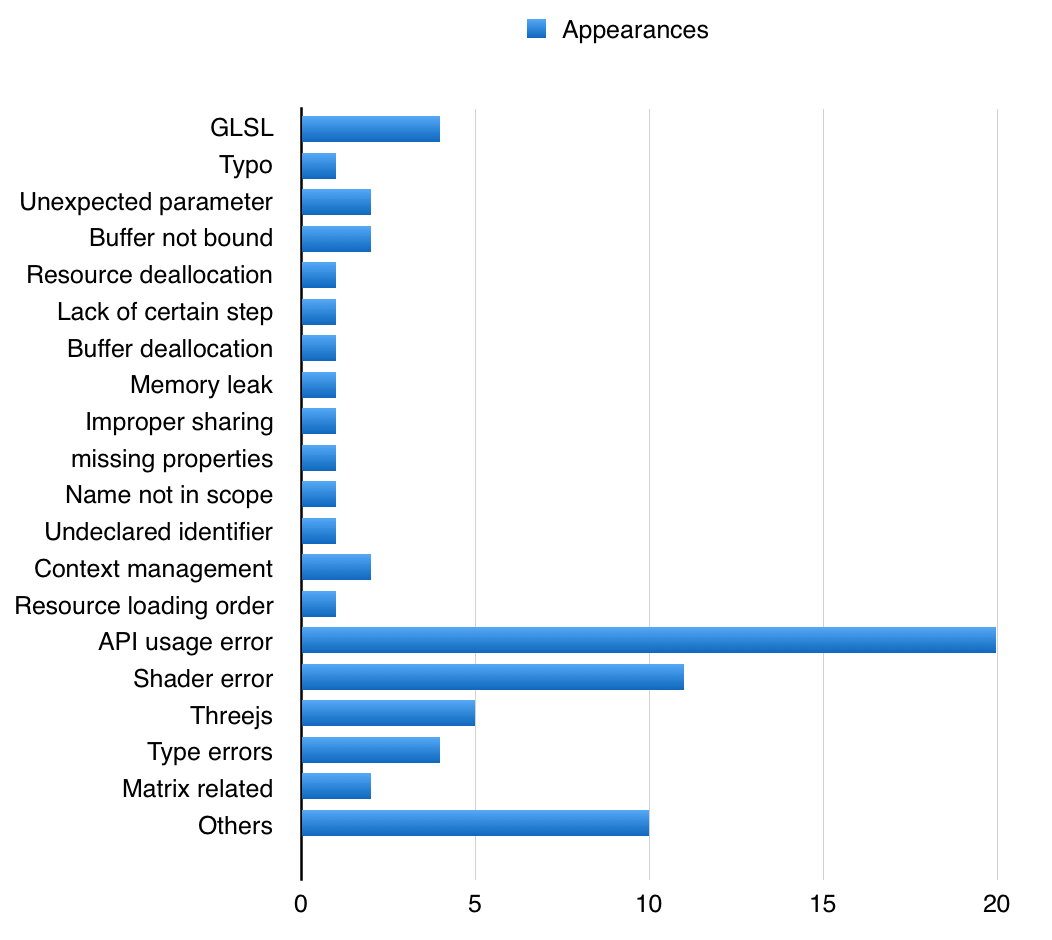
\includegraphics{images/apperances.png}
\end{figure}

\newpage
\section{Library Support}\label{library-support}

\subsection{Overview}\label{overview-2}

\subsubsection{Popular libraries}\label{popular-libraries}

\begin{itemize}
\itemsep1pt\parskip0pt\parsep0pt
\item
  High-level libraries: BabylonJS, three.js, O3D, OSG.JS, CopperLicht
  and GLGE
\item
  Matrix libraries: gl-matrix, sylvester
\end{itemize}

\subsubsection{Abstractions}\label{abstractions}

Take three.js as an example:

\begin{itemize}
\itemsep1pt\parskip0pt\parsep0pt
\item
  Geometry
\item
  Objects
\item
  Materials
\item
  Lights
\item
  Resource loaders
\item
  Linear algebra
\item
  Scenes
\item
  Camera
\item
  Renderer (not just WebGL)
\item
  Textures
\end{itemize}

\subsubsection{Why libraries?}\label{why-libraries}

\begin{enumerate}
\def\labelenumi{\arabic{enumi}.}
\itemsep1pt\parskip0pt\parsep0pt
\item
  The developer can focus on the logic of their applications/business,
  rather than the implementation details;
\item
  The third-party library's APIs are better designed to fit the language
  construct of JavaScript
\item
  The high-level library is simpler and more restricted in effects --
  which means less error-prone.
\end{enumerate}

As a result, the following errors can be eliminated by using a library:

\begin{itemize}
\itemsep1pt\parskip0pt\parsep0pt
\item
  Typo
\item
  Buffer binding
\item
  Resource Management
\item
  Lack of certain step
\item
  Missing properties
\item
  Name not in scope
\item
  Undeclared identifier
\item
  API usage error
\item
  Matrix related
\end{itemize}

\subsection{Case study: gl-matrix}\label{case-study-gl-matrix}

\href{http://glmatrix.net}{Home}

glMatrix is designed to perform vector and matrix operations stupidly
fast! The latest version uses WebPack to manage the modules.

\subsubsection{APIs}\label{apis}

Exposed interfaces: \texttt{glMatrix}, \texttt{mat2}, \texttt{mat2d},
\texttt{mat3}, \texttt{mat4}, \texttt{quat}, \texttt{vec2},
\texttt{vec3}, \texttt{vec4}

\paragraph{\href{http://glmatrix.net/docs/2.2.0/symbols/glMatrix.html}{Common
utilities}}\label{common-utilities}

\begin{figure}[htbp]
\centering
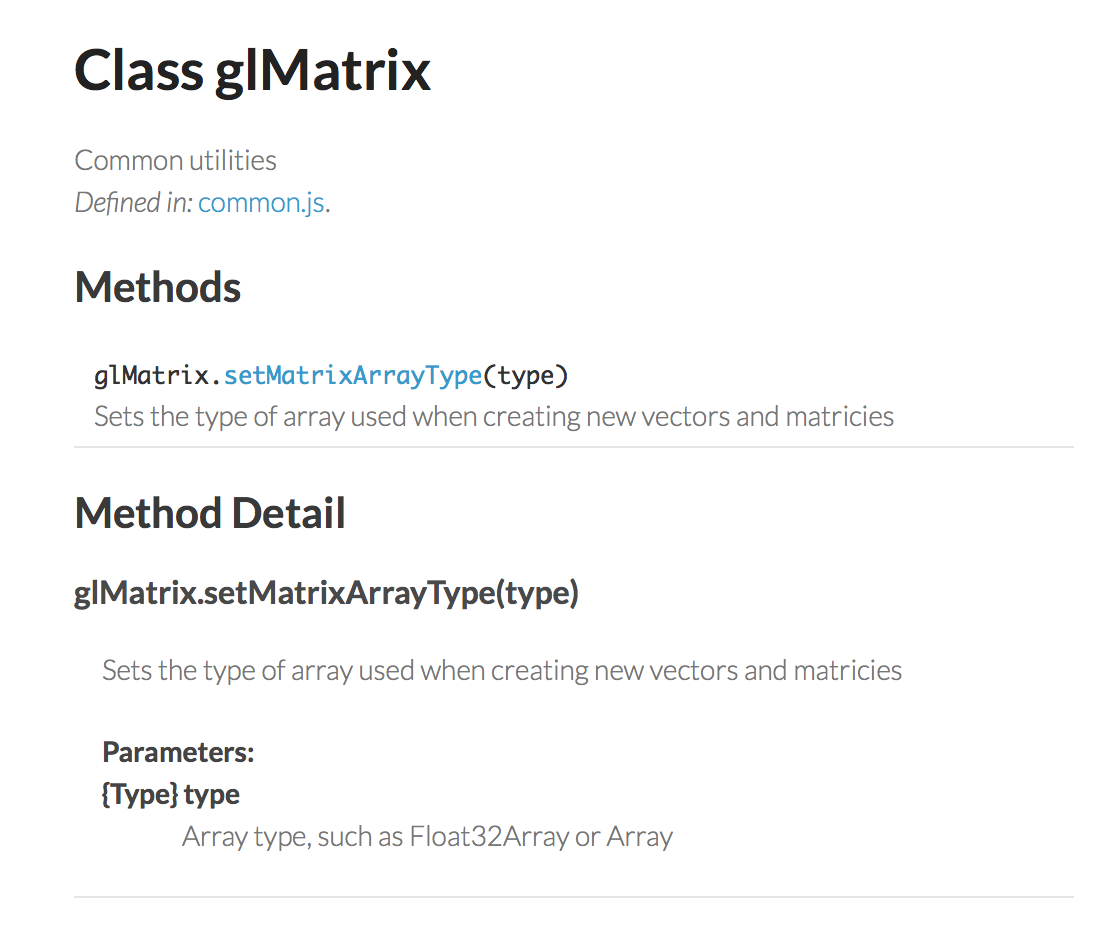
\includegraphics{images/gl-matrix.png}
\end{figure}

\paragraph{\href{http://glmatrix.net/docs/2.2.0/symbols/mat3.html}{3x3
Matrix}}\label{x3-matrix}

\begin{figure}[htbp]
\centering
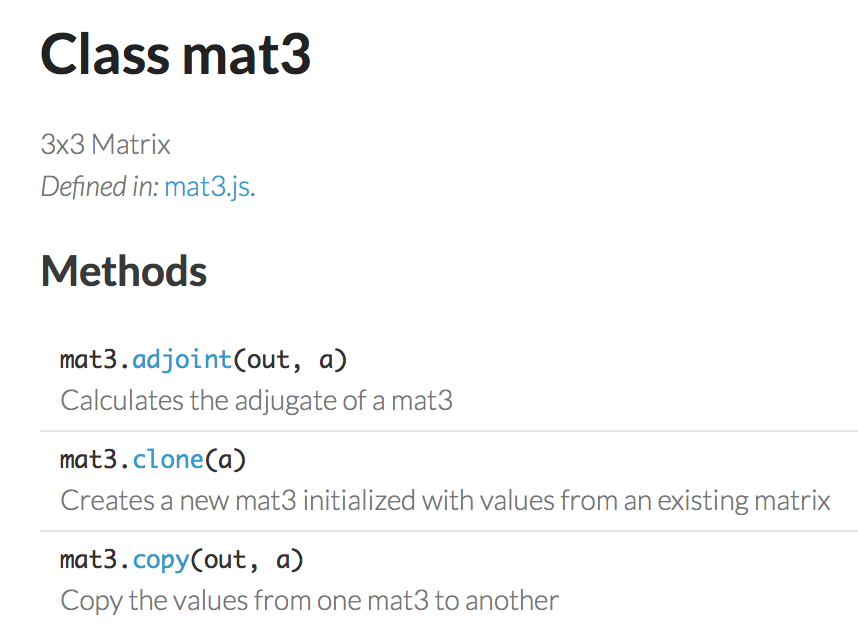
\includegraphics{images/mat3.png}
\end{figure}

\begin{figure}[htbp]
\centering
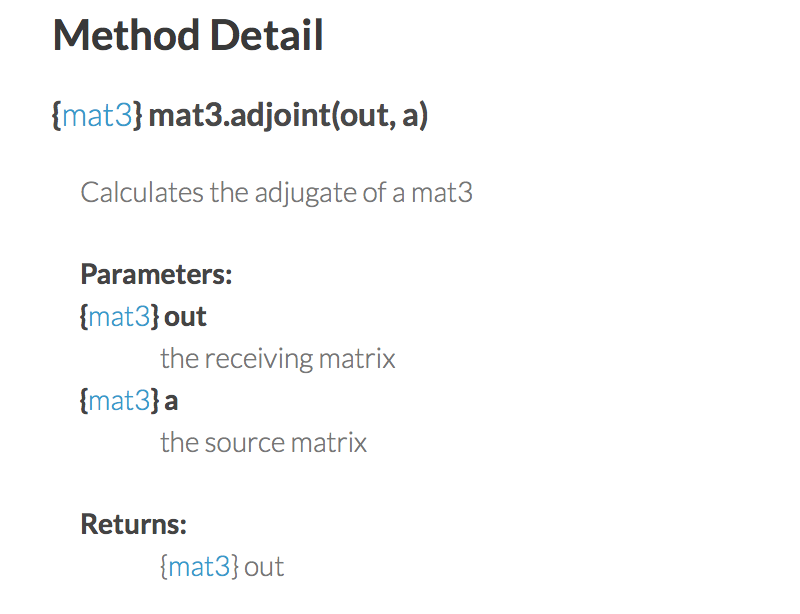
\includegraphics{images/mat3-adjoint.png}
\end{figure}

\subsubsection{Library structure}\label{library-structure}

\begin{itemize}
\itemsep1pt\parskip0pt\parsep0pt
\item
  \texttt{glMatrix}: Common utilities, including config constants,
  compatibility detection, and things like \texttt{setMatrixArrayType}.
\item
  \texttt{mat3} etc: Represent one type of data and the related
  operations.

  \begin{itemize}
  \itemsep1pt\parskip0pt\parsep0pt
  \item
    Constructors: \texttt{create}, \texttt{clone}, \texttt{copy}
  \item
    Computations: \texttt{identity}, \texttt{transpose}
  \item
    Conversions: \texttt{fromMat4}
  \end{itemize}
\end{itemize}

\subsubsection{Possible problems}\label{possible-problems}

\begin{enumerate}
\def\labelenumi{\arabic{enumi}.}
\itemsep1pt\parskip0pt\parsep0pt
\item
  \textbf{Hard to maintain}: Even such a simple library is over 6000
  lines of JS; and the author suggested a ``sorry'' for breaking the
  APIs from 1.0 to 2.0.
\item
  \textbf{Type Unsafe}: Concretely, it is easy to pass a \texttt{vec3}
  to where a \texttt{vec4} is expected. And since here is no type
  checking, so you won't get any explicit warning.
\end{enumerate}

\subsection{Case Study: Threejs}\label{case-study-threejs}

\subsubsection{API samples}\label{api-samples}

\href{http://threejs.org/docs/}{Docs}

A example app, its workflow:

\begin{itemize}
\itemsep1pt\parskip0pt\parsep0pt
\item
  initialize \texttt{scene}, \texttt{camera} and \texttt{renderer}.
\item
  Create mesh object from geometry and material add them to the scene
\item
  Render based on scene and camera frame by frame
\end{itemize}

\begin{Shaded}
\begin{Highlighting}[]
\KeywordTok{<html>}
    \KeywordTok{<head>}
        \KeywordTok{<title>}\NormalTok{My first Three.js app}\KeywordTok{</title>}
        \KeywordTok{<style>}
            \NormalTok{body }\KeywordTok{\{} \KeywordTok{margin:} \DataTypeTok{0}\KeywordTok{;} \KeywordTok{\}}
            \NormalTok{canvas }\KeywordTok{\{} \KeywordTok{width:} \DataTypeTok{100%}\KeywordTok{;} \KeywordTok{height:} \DataTypeTok{100%} \KeywordTok{\}}
        \KeywordTok{</style>}
    \KeywordTok{</head>}
    \KeywordTok{<body>}
        \KeywordTok{<script}\OtherTok{ src=}\StringTok{"js/three.min.js"}\KeywordTok{></script>}
        \KeywordTok{<script>}
            \KeywordTok{var} \NormalTok{scene = }\KeywordTok{new} \OtherTok{THREE}\NormalTok{.}\FunctionTok{Scene}\NormalTok{();}
            \KeywordTok{var} \NormalTok{camera = }\KeywordTok{new} \OtherTok{THREE}\NormalTok{.}\FunctionTok{PerspectiveCamera}\NormalTok{( }\DecValTok{75}\NormalTok{,}
                             \OtherTok{window}\NormalTok{.}\FunctionTok{innerWidth}\NormalTok{/}\OtherTok{window}\NormalTok{.}\FunctionTok{innerHeight}\NormalTok{, }\FloatTok{0.1}\NormalTok{, }\DecValTok{1000} \NormalTok{);}

            \KeywordTok{var} \NormalTok{renderer = }\KeywordTok{new} \OtherTok{THREE}\NormalTok{.}\FunctionTok{WebGLRenderer}\NormalTok{();}
            \OtherTok{renderer}\NormalTok{.}\FunctionTok{setSize}\NormalTok{( }\OtherTok{window}\NormalTok{.}\FunctionTok{innerWidth}\NormalTok{, }\OtherTok{window}\NormalTok{.}\FunctionTok{innerHeight} \NormalTok{);}
            \OtherTok{document}\NormalTok{.}\OtherTok{body}\NormalTok{.}\FunctionTok{appendChild}\NormalTok{( }\OtherTok{renderer}\NormalTok{.}\FunctionTok{domElement} \NormalTok{);}

            \KeywordTok{var} \NormalTok{geometry = }\KeywordTok{new} \OtherTok{THREE}\NormalTok{.}\FunctionTok{BoxGeometry}\NormalTok{( }\DecValTok{1}\NormalTok{, }\DecValTok{1}\NormalTok{, }\DecValTok{1} \NormalTok{);}
            \KeywordTok{var} \NormalTok{material = }\KeywordTok{new} \OtherTok{THREE}\NormalTok{.}\FunctionTok{MeshBasicMaterial}\NormalTok{( \{ }\DataTypeTok{color}\NormalTok{: }\BaseNTok{0x00ff00} \NormalTok{\} );}
            \KeywordTok{var} \NormalTok{cube = }\KeywordTok{new} \OtherTok{THREE}\NormalTok{.}\FunctionTok{Mesh}\NormalTok{( geometry, material );}
            \OtherTok{scene}\NormalTok{.}\FunctionTok{add}\NormalTok{( cube );}

            \OtherTok{camera}\NormalTok{.}\OtherTok{position}\NormalTok{.}\FunctionTok{z} \NormalTok{= }\DecValTok{5}\NormalTok{;}

            \KeywordTok{var} \NormalTok{render = }\KeywordTok{function} \NormalTok{() \{}
                \FunctionTok{requestAnimationFrame}\NormalTok{( render );}

                \OtherTok{cube}\NormalTok{.}\OtherTok{rotation}\NormalTok{.}\FunctionTok{x} \NormalTok{+= }\FloatTok{0.1}\NormalTok{;}
                \OtherTok{cube}\NormalTok{.}\OtherTok{rotation}\NormalTok{.}\FunctionTok{y} \NormalTok{+= }\FloatTok{0.1}\NormalTok{;}

                \OtherTok{renderer}\NormalTok{.}\FunctionTok{render}\NormalTok{(scene, camera);}
            \NormalTok{\};}

            \FunctionTok{render}\NormalTok{();}
        \NormalTok{<}\OtherTok{/script>}
\OtherTok{    </body}\NormalTok{>}
\NormalTok{<}\OtherTok{/html>}
\end{Highlighting}
\end{Shaded}


\subsubsection{Library structure}\label{library-structure-1}

\begin{quote}
The current three.js implementation is too huge -- I will take its early
release \texttt{three.js-r16} as a preliminary analysis object.
\end{quote}

The \texttt{src} contains

\begin{enumerate}
\def\labelenumi{\arabic{enumi}.}
\itemsep1pt\parskip0pt\parsep0pt
\item
  cameras: set up the perspective matrix etc. based on camera paramters
\item
  core

  \begin{enumerate}
  \def\labelenumii{\arabic{enumii}.}
  \itemsep1pt\parskip0pt\parsep0pt
  \item
    Color: convert hexadecimal code into internal representation and
    better format
  \item
    Face3/Face4: Wrap end-points and normal vector into a high-level
    structure \texttt{Face}
  \item
    Geometry: A geometry is a set of vertices and faces connecting the
    vertices, this function computes the normals of each face (which
    might be useful in texture or fragment shader?)
  \item
    Vector(2, 3, 4)/Matrix4: Basically same as \texttt{gl-matrix}
  \item
    Vertex: Wrapper over position and normal (normal?)
  \item
    UV: (u, v) coordinate (NOTE: UV mapping is a process of flattening
    the 3-dimensional object)
  \item
    Rectangle: Again, a geometry wrapper
  \end{enumerate}
\item
  materials: Wrap the attribute values of different materials
\item
  objects: Simple wrappers of \texttt{Line}, \texttt{Mesh},
  \texttt{Object3D} etc.
\item
  renderers

  \begin{enumerate}
  \def\labelenumii{\arabic{enumii}.}
  \itemsep1pt\parskip0pt\parsep0pt
  \item
    \texttt{renderables}: \texttt{RendererableFace(3,4)},
    \texttt{RenderableLine}, \texttt{RenderableParticle} etc., looks
    like another set of wrappers
  \item
    \texttt{CanvasRenderer}: In construction, context is get from
    created \texttt{canvas} element; A lot of other vectors and
    rectangle are created as well. The functions provided include
    \texttt{setSize}, \texttt{clear}, \texttt{render},
    \texttt{drawTexturedTriangle} and \texttt{expand}. However, this is
    only a 2d canvas.
  \item
    \texttt{Renderer}: Its data includes pools of face3, face4, line and
    particles, as well as a vector4 and a matrix4. The exposed
    interfaces include a \texttt{renderList} and method
    \texttt{project}. I suppose that this will do some transformation
    (like projection), and push the things left to render into
    \texttt{renderList}
  \item
    \texttt{SVGRenderer}: Similar to \texttt{CanvasRenderer}
  \item
    \texttt{WebGLRenderer}: Similar to \texttt{CanvasRenderer}, we have
    some basic bootstrapping and after that, we call \texttt{initGL} and
    \texttt{initProgram}; The utilities provided include
    \texttt{setSize}, \texttt{clear} \texttt{render},
    \texttt{getShader}; There are also internal functions
    \texttt{getShader} and \texttt{matrix2Array}.

    \begin{itemize}
    \itemsep1pt\parskip0pt\parsep0pt
    \item
      \texttt{initGL}: It will try to get context, and will throw in
      case of incompatibility. If context is ready, it will do
      \texttt{clearColor}, \texttt{clearDepth} and other config and
      setups.
    \item
      \texttt{initProgram}: Two shaders, fragment and vertex shaders are
      hard-coded here. With attached shaders, it link and use the
      program. Finally, it will set other attributes related.
    \item
      \texttt{clear}: Clear the \texttt{COLOR\_BUFFER\_BIT} and
      \texttt{DEPTH\_BUFFER\_BIT} bits.
    \item
      \texttt{render}: Given a \texttt{scene} and a \texttt{camera}, it
      will render the mesh object in \texttt{scene} one by one. Every
      mesh object will have its vertex buffer. The related data also
      contains faces and color. For every face, its three vertices will
      be push into the array, same for color. With buffers ready, it
      will create, bind and fill in one by one with
      \texttt{createBuffer}, \texttt{bindBuffer} and
      \texttt{bufferData}. After that, the view matrix and projection
      matrix is set. Next, the material of object is rendered as well.
      The color of face are pushed into the buffer, bind and filled in.
      Finally, we will call \texttt{drawElements}.
    \item
      \texttt{getShader}: It is basically wrapping around
      \texttt{createShader}, \texttt{shaderSource},
      \texttt{compileShader}.
    \end{itemize}
  \end{enumerate}
\item
  scenes: Wrapper of an array of objects
\end{enumerate}

\newpage
\section{Tool Support}\label{tool-support}

\subsection{Exclusive Debug tools}\label{exclusive-debug-tools}

\begin{quote}
Some debugging tools for WebGL development are listed here.
\end{quote}

\href{http://www.realtimerendering.com/blog/webgl-debugging-and-profiling-tools/}{Another
post}

\subsubsection{WebGL Insights}\label{webgl-insights}

\href{https://github.com/3Dparallax/insight}{Home}

This tool looks very powerful and mature. Look at the features:

\begin{itemize}
\itemsep1pt\parskip0pt\parsep0pt
\item
  Chrome Extension embedded in the Chrome DevTools panel
\item
  Overdraw Inspector
\item
  Mipmap Inspector
\item
  Depth Inspector
\item
  Call Stack Timeline and Statistics
\item
  Program Usage Count
\item
  Duplicate Program Usage Detector
\item
  Program Viewer
\item
  Frame Control
\item
  State Variable Editor
\item
  Resource Viewer
\end{itemize}

One screen-shot:

\begin{figure}[htbp]
\centering
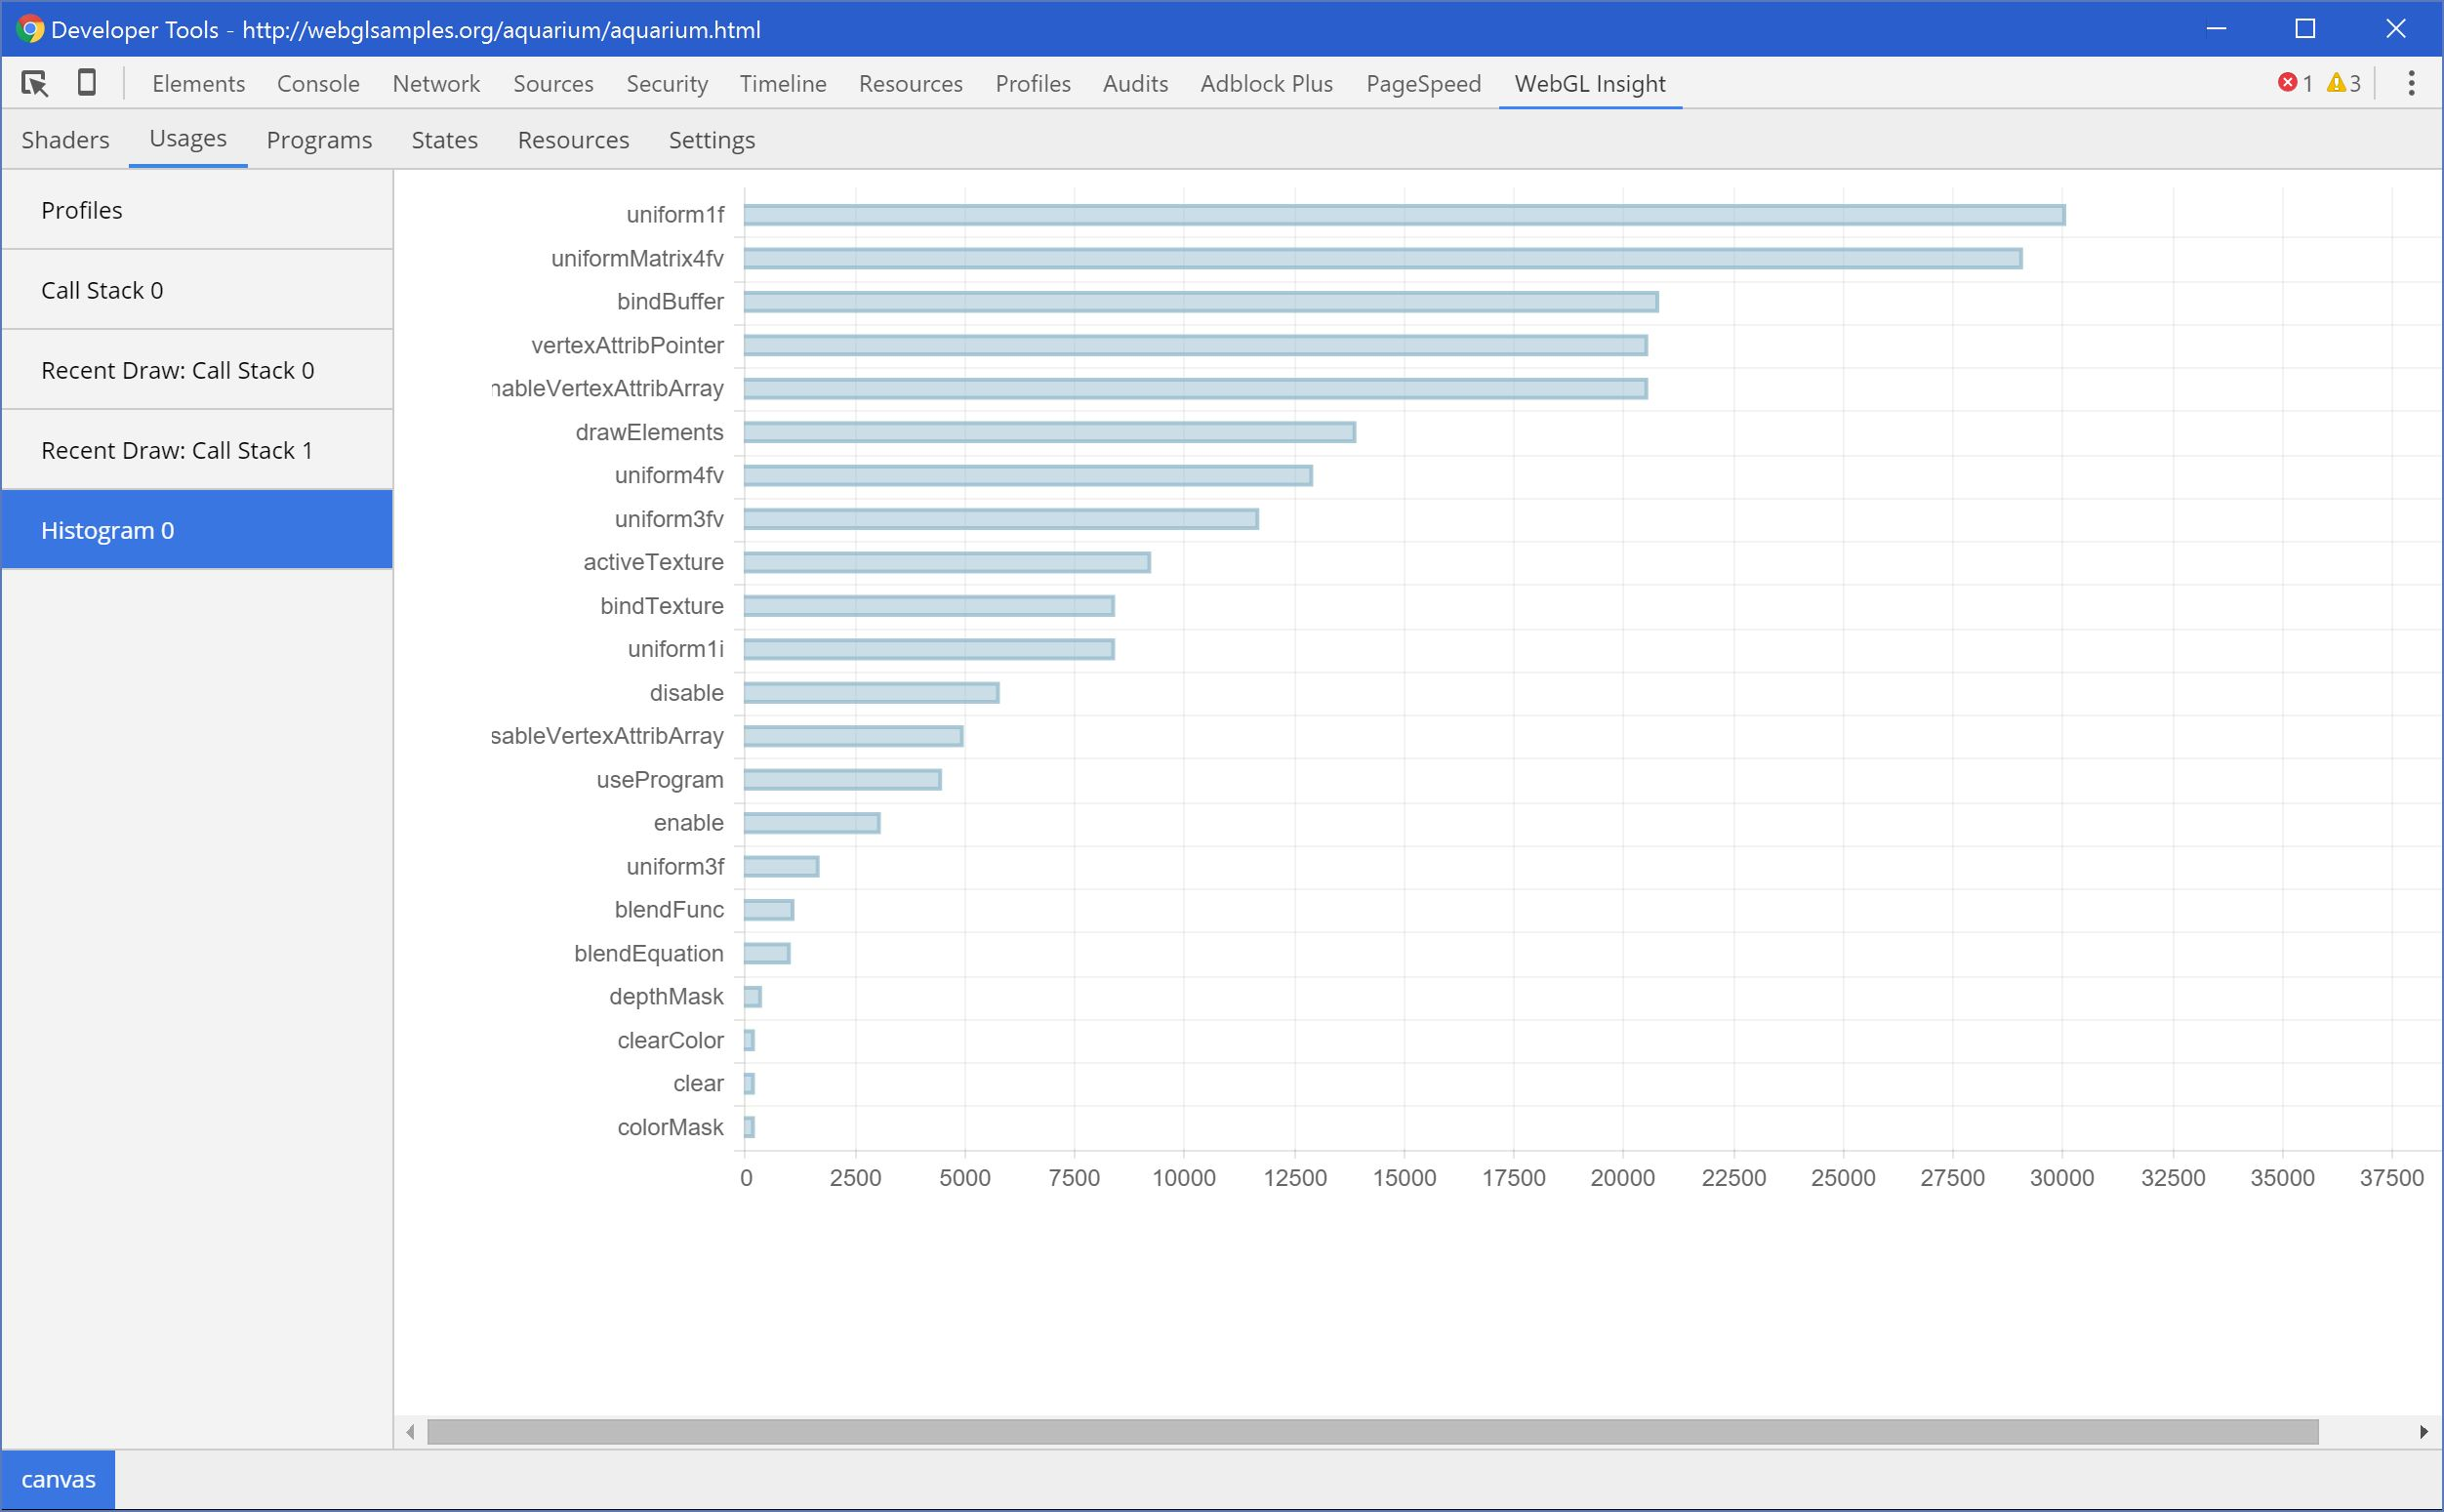
\includegraphics{images/inspector.jpeg}
\end{figure}

\subsubsection{WebGL-Inspector}\label{webgl-inspector}

\href{https://benvanik.github.com/WebGL-Inspector/}{Home}

Features

\begin{itemize}
\itemsep1pt\parskip0pt\parsep0pt
\item
  Extension for injecting into pages
\item
  Embed in an existing application with a single script include
\item
  Capture entire GL frames
\item
  Annotated call log with stepping/resource navigation and redundant
  call warnings
\item
  Pixel history - see all draw calls that contributed to a pixel +
  blending information
\item
  GL state display
\item
  Resource browsers for textures, buffers, and programs
\end{itemize}

\href{http://benvanik.github.io/WebGL-Inspector/samples/lesson05/embedded.html}{Demo}

\begin{figure}[htbp]
\centering
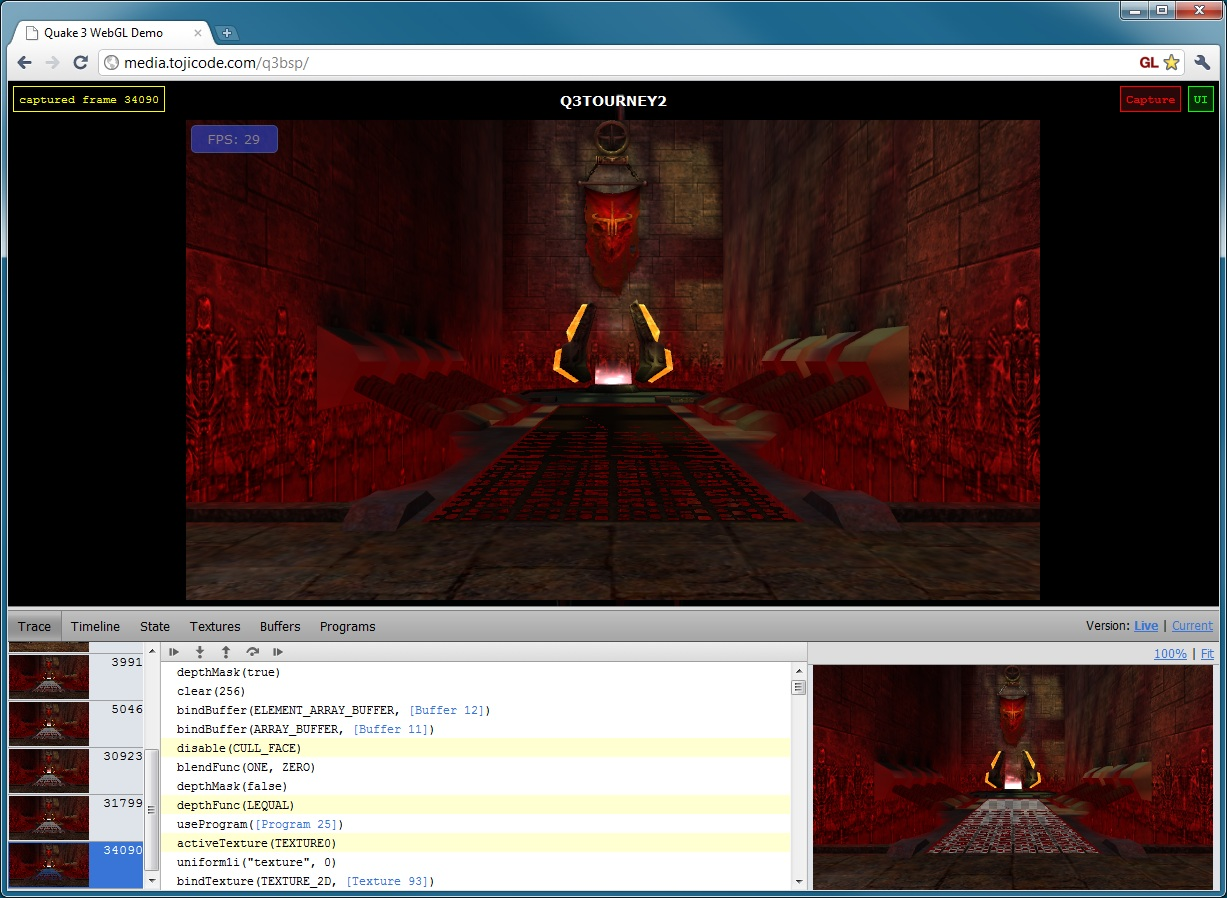
\includegraphics{images/inspector2.jpg}
\end{figure}

This is a very convenient debugger, it can be useful when you
application's logic is wrong (compared to our analyzer's target -- the
syntax and API is wrong).

\subsubsection{webgl-debug.js}\label{webgl-debug.js}

\begin{itemize}
\itemsep1pt\parskip0pt\parsep0pt
\item
  \href{https://github.com/KhronosGroup/WebGLDeveloperTools}{Repo}
\item
  \href{https://www.khronos.org/webgl/wiki/Debugging}{Home}
\end{itemize}

It will wrap the \texttt{WebGLRenderingContext} with a debugging
wrapper, which will make any GL errors show up in the JavaScript console
of browser.

Also, we can log function calls with by passing a logger in the above
mentioned wrapper.

It provides
\href{https://github.com/KhronosGroup/WebGLDeveloperTools/blob/master/src/debug/debug-sample.html}{a
sample}.

\subsubsection{WebGL Linter}\label{webgl-linter}

\href{https://github.com/CharlesLillo/WebGL_Linter}{Repo}

This is a discontinued and very primitive project -- but the idea is
there. \#\# Browser Support and IDE Support

\subsubsection{Browser}\label{browser}

\paragraph{Chrome Canvas Inspector}\label{chrome-canvas-inspector}

See
\href{http://learningthreejs.com/blog/2013/04/05/debugging-with-chromes-canvas-inspection/}{the
post}

\paragraph{Firefox Shader Editor}\label{firefox-shader-editor}

See
\href{https://hacks.mozilla.org/2013/11/live-editing-webgl-shaders-with-firefox-developer-tools/}{this
post}

\subsubsection{IDE}\label{ide}

Generally speaking, by using an IDE, you can avoid a lot of silly bugs
all-together.

Also, there are some graphical editors for modeling.

\paragraph{JetBrain - WebStorm}\label{jetbrain---webstorm}

It has \href{https://plugins.jetbrains.com/plugin/6993?pr=idea}{support
for GLSL language by plugin}.

\paragraph{WebGL Studio}\label{webgl-studio}

\href{http://webglstudio.org}{Home}

\paragraph{Three.js editor}\label{three.js-editor}

\href{http://threejs.org/editor/}{Home}

\paragraph{3Dmol.js}\label{dmol.js}

\href{http://3dmol.csb.pitt.edu}{Home}

\paragraph{Blend4Web}\label{blend4web}

\href{https://www.blend4web.com/en/}{Home}

\newpage
\section{Conclusion}\label{conclusion}

\subsection{Best practices in WebGL
development}\label{best-practices-in-webgl-development}

\subsubsection{General ones}\label{general-ones}

\begin{enumerate}
\def\labelenumi{\arabic{enumi}.}
\itemsep1pt\parskip0pt\parsep0pt
\item
  If you are writing code -- Use a good IDE or modern editor, such as
  WebStorm, Eclipse, and Atom. This can help you prevent most silly
  errors when you are still a newbie.
\item
  Use the graphical editor to get your model (in fact, you can model in
  softwares like Blender and Maya, then import the model into the JS).
\item
  Make error explicit -- Check return value always, catch possible
  errors.
\item
  Take advantages of debugging tools like WebGL inspector.
\end{enumerate}

\subsubsection{Technical ones}\label{technical-ones}

\begin{itemize}
\itemsep1pt\parskip0pt\parsep0pt
\item
  \href{https://developer.mozilla.org/en-US/docs/Web/API/WebGL_API/WebGL_best_practices}{Article
  from MDN}
\item
  \href{https://github.com/glQuery/webgl-best-practices}{glQuery/webgl-best-practices}
\end{itemize}

\subsection{Future of WebGL tooling}\label{future-of-webgl-tooling}

\subsubsection{Static analysis
technique}\label{static-analysis-technique}

The interoperation between JavaScript and GLSL opens a door for static
analysis; Besides, editors and current IDE is unaware of if you have
check \texttt{null}; The dynamic type information is simply ignored.

Also, the correct use of API involves side-effects, which is easy to get
wrong.

\subsubsection{Verified libraries}\label{verified-libraries}

Three.js is a huge code base, and highly dynamic. You never know if some
feature does work or it is just coincidence.

By verifying:

\begin{enumerate}
\def\labelenumi{\arabic{enumi}.}
\itemsep1pt\parskip0pt\parsep0pt
\item
  The library does what it is intended to do
\item
  The library does its job the right way
\end{enumerate}

We will have more confidence and rely on it in the long run.

\subsubsection{Integration}\label{integration}

The integration into mature product is important, such as debug tools
and IDEs.

\bibliographystyle{plain}
\bibliography{main}


\end{document}
